\documentclass{article}

\usepackage{amsmath, amsthm, amssymb, amsfonts}
\usepackage{thmtools}
\usepackage{graphicx}
\usepackage{setspace}
\usepackage{geometry}
\usepackage{float}
\usepackage{hyperref}
\usepackage[utf8]{inputenc}
\usepackage[english]{babel}
\usepackage{framed}
\usepackage[dvipsnames]{xcolor}
\usepackage{tcolorbox}
\usepackage{tabularx}
\usepackage{longtable}

\colorlet{LightGray}{White!90!Periwinkle}
\colorlet{LightOrange}{Orange!15}
\colorlet{LightGreen}{Green!15}

\newcommand{\HRule}[1]{\rule{\linewidth}{#1}}

\declaretheoremstyle[name=Theorem,]{thmsty}
\declaretheorem[style=thmsty,numberwithin=section]{theorem}
\tcolorboxenvironment{theorem}{colback=LightGray}

\declaretheoremstyle[name=Proposition,]{prosty}
\declaretheorem[style=prosty,numberlike=theorem]{proposition}
\tcolorboxenvironment{proposition}{colback=LightOrange}

\declaretheoremstyle[name=Principle,]{prcpsty}
\declaretheorem[style=prcpsty,numberlike=theorem]{principle}
\tcolorboxenvironment{principle}{colback=LightGreen}

\setstretch{1.2}
\geometry{
    textheight=9in,
    textwidth=5.5in,
    top=1in,
    headheight=12pt,
    headsep=25pt,
    footskip=30pt
}

\begin{document}

% ------------------------------------------------------------------------------
% Cover Page and ToC
% ------------------------------------------------------------------------------

\title{ \normalsize \textsc{}
\\ [2.0cm]
\HRule{1.5pt} \\
\LARGE \textbf{\uppercase{Documento de Casos de Uso}
\HRule{2.0pt} \\ [0.6cm] \LARGE{Sistema de Conciliaciones Bancarias} \vspace*{10\baselineskip}}
}
\date{}
\author{\textbf{Ricardo Emmanuel Uriegas Ibarra}}

\maketitle
% remove page number from the cover page
\thispagestyle{empty} % Quita el número de página en esta página
\newpage

\tableofcontents
\newpage

% ---------------------------------------------------------------------------- %
% Document Content
% ---------------------------------------------------------------------------- %
\section{Introducción}

\subsection{Propósito del documento}
Este documento tiene como objetivo describir los requisitos funcionales y no funcionales del Sistema de Conciliaciones Bancarias. Su propósito principal es apoyar a los auditores en su labor, facilitando la revisión y validación de movimientos bancarios.

\subsection{Alcance del sistema}
El sistema permitirá gestionar múltiples cuentas bancarias, registrar ingresos y egresos, realizar conciliaciones bancarias comparativas y generar reportes detallados para apoyar en auditorías. Está diseñado para un número ilimitado de auditores y optimiza los procesos de conciliación y análisis financiero.

\newpage
\section{Requisitos Funcionales}

\subsection{RF1. Iniciar Sesión}
\begin{itemize}
    \item \textbf{Descripción:} El sistema permitirá a los usuarios autenticarse ingresando sus credenciales.
    \item \textbf{Regla:} Las credenciales ingresadas deben ser verificadas y validadas antes de otorgar acceso. En caso de credenciales incorrectas, se mostrará un mensaje de error.
\end{itemize}

\subsection{RF2. Cerrar Sesión}
\begin{itemize}
    \item \textbf{Descripción:} Los usuarios podrán cerrar sesión de manera segura en el sistema.
    \item \textbf{Regla:} Al cerrar sesión, se debe invalidar la sesión activa y garantizar la seguridad de los datos del usuario.
\end{itemize}

\subsection{RF3. Gestión de Usuarios}
\begin{itemize}
    \item \textbf{Descripción:} El sistema permitirá a los administradores agregar, modificar y eliminar usuarios.
    \item \textbf{Regla:} Solo los administradores podrán acceder a esta funcionalidad. Se deben ingresar los datos forzosos al crear o modificar un usuario:
    \begin{itemize}
        \item Nombre completo
        \item Número de folio de credencial de elector o número de INE
        \item Fecha de nacimiento
        \item Número de cédula profesional
        \item Dirección
        \item Teléfono
        \item Correo electrónico
        \item Sexo
    \end{itemize}
    \item \textbf{Nota:} Los datos no forzosos como edad y peso son opcionales.
\end{itemize}

\subsection{RF4. Gestión de Cuentas Bancarias}
\begin{itemize}
    \item \textbf{Descripción:} El sistema permitirá a los administradores agregar, modificar y eliminar cuentas bancarias.
    \item \textbf{Regla:} Cada cuenta bancaria debe estar asociada a un usuario válido en el sistema.
\end{itemize}

\subsection{RF5. Gestión de Ingresos y Egresos}
\begin{itemize}
    \item \textbf{Descripción:} El sistema permitirá registrar, modificar y eliminar ingresos y egresos asociados a cuentas bancarias.
    \item \textbf{Regla:} Solo los administradores y auditores podrán realizar estas operaciones. Se debe validar la información antes de guardarla en la base de datos.
\end{itemize}

\subsection{RF6. Conciliación Bancaria}
\begin{itemize}
    \item \textbf{Descripción:} El sistema permitirá realizar la conciliación bancaria comparando ingresos y egresos internos con el estado de cuenta bancario. Adicionalmente, se comparará el saldo total con el libro contable.
    \item \textbf{Regla:} La conciliación incluirá:
    \begin{itemize}
        \item Periodo de tiempo (fecha de inicio y término)
        \item Saldo inicial del libro contable del mes anterior
        \item Comparación de movimientos internos contra movimientos externos
    \end{itemize}
    \item \textbf{Nota:} Los movimientos ya conciliados no podrán ser modificados.
\end{itemize}

\subsection{RF7. Generación de Reportes}
\begin{itemize}
    \item \textbf{Descripción:} Los auditores podrán generar reportes detallados de movimientos conciliados y pendientes.
    \item \textbf{Regla:} Los reportes estarán disponibles en formatos como PDF y Excel para facilitar su análisis y presentación.
\end{itemize}

\subsection{RF8. Consulta del Libro Contable}
\begin{itemize}
    \item \textbf{Descripción:} El sistema permitirá consultar el libro contable, mostrando todos los movimientos registrados y el saldo total.
    \item \textbf{Regla:} Se podrán aplicar filtros por fecha, tipo de movimiento y otros criterios para una mejor visualización.
\end{itemize}

\subsection{RF9. Seguridad de Acceso}
\begin{itemize}
    \item \textbf{Descripción:} El sistema implementará autenticación y autorización para controlar el acceso a las funcionalidades.
    \item \textbf{Regla:} Las contraseñas deben estar encriptadas y se utilizará un middleware para gestionar la seguridad. Solo los usuarios con permisos adecuados podrán acceder a ciertas funcionalidades.
\end{itemize}

\newpage
\section{Requisitos No Funcionales}

\subsection{RNF1. Seguridad}
\begin{itemize}
    \item \textbf{Descripción:} El sistema debe garantizar la seguridad de la información y las comunicaciones entre el cliente y el servidor.
    \item \textbf{Regla:} Se deben implementar las siguientes medidas:
    \begin{itemize}
        \item Uso de HTTPS para todas las comunicaciones.
        \item Implementación de middleware de seguridad para proteger la base de datos y las aplicaciones.
    \end{itemize}
\end{itemize}

\subsection{RNF2. Rendimiento}
\begin{itemize}
    \item \textbf{Descripción:} El sistema debe responder de manera eficiente a las acciones del usuario.
    \item \textbf{Regla:} Las operaciones más comunes deben ejecutarse en un tiempo máximo de 2 segundos para no afectar la experiencia del usuario.
\end{itemize}

\subsection{RNF3. Usabilidad}
\begin{itemize}
    \item \textbf{Descripción:} La interfaz de usuario debe ser intuitiva y fácil de usar, facilitando las tareas de administradores y auditores.
    \item \textbf{Regla:} Se deben seguir las buenas prácticas de diseño de interfaz y experiencia de usuario, ofreciendo ayuda en línea y mensajes claros.
\end{itemize}

\subsection{RNF4. Compatibilidad}
\begin{itemize}
    \item \textbf{Descripción:} El sistema debe ser compatible con los principales navegadores web y dispositivos.
    \item \textbf{Regla:} Debe funcionar correctamente en las últimas versiones de Chrome, Firefox, Edge y Safari, así como en dispositivos móviles y tablets.
\end{itemize}

\subsection{RNF5. Mantenibilidad}
\begin{itemize}
    \item \textbf{Descripción:} El sistema debe ser fácil de mantener y actualizar.
    \item \textbf{Regla:} El código debe estar bien documentado y estructurado siguiendo estándares de programación para facilitar futuras modificaciones.
\end{itemize}

\subsection{RNF6. Escalabilidad}
\begin{itemize}
    \item \textbf{Descripción:} El sistema debe poder manejar un aumento en la cantidad de usuarios y datos sin degradar su rendimiento.
    \item \textbf{Regla:} La arquitectura del sistema debe permitir la adición de recursos y la distribución de carga si es necesario.
\end{itemize}

\subsection{RNF7. Integridad y Confidencialidad de Datos}
\begin{itemize}
    \item \textbf{Descripción:} La información almacenada debe mantenerse íntegra y confidencial.
    \item \textbf{Regla:} Se deben implementar backups periódicos y controlar el acceso a la información según los perfiles de usuario.
\end{itemize}

\subsection{RNF8. Disponibilidad}
\begin{itemize}
    \item \textbf{Descripción:} El sistema debe estar disponible para los usuarios siempre que sea necesario.
    \item \textbf{Regla:} El tiempo de inactividad planificado debe ser mínimo y, preferiblemente, programado fuera de las horas laborales.
\end{itemize}

\newpage
\section{Casos de Uso}
\subsection{CU1: Iniciar Sesión}
\begin{longtable}{|l|p{10cm}|}
\hline
\textbf{Actor} & Usuario (Administrador o Auditor) \\ \hline
\textbf{Descripción} & El usuario inicia sesión en el sistema proporcionando sus credenciales para acceder a las funcionalidades según su rol. \\ \hline
\textbf{Precondiciones} & 
\begin{itemize}
    \item El usuario debe estar registrado en el sistema.
    \item El usuario debe tener sus credenciales (correo electrónico y contraseña) activas.
\end{itemize} \\ \hline
\textbf{Flujo Principal} & 
\begin{enumerate}
    \item El usuario accede a la pantalla de inicio de sesión.
    \item El usuario ingresa su correo electrónico y contraseña.
    \item El sistema valida las credenciales ingresadas.
    \item El sistema verifica el rol del usuario (Administrador o Auditor).
    \item El sistema permite el acceso y redirige al usuario al menú principal correspondiente a su rol.
\end{enumerate} \\ \hline
\textbf{Excepciones} & 
\begin{itemize}
    \item \textbf{E1: Credenciales Incorrectas}
    \begin{enumerate}
        \item[3a.] Si las credenciales son incorrectas, el sistema muestra un mensaje de error indicando que el correo electrónico o contraseña son inválidos.
        \item[3b.] El usuario puede intentar iniciar sesión nuevamente.
    \end{enumerate}
    \item \textbf{E2: Cuenta Bloqueada}
    \begin{enumerate}
        \item[3a.] Si el usuario excede el número máximo de intentos fallidos (3 intentos), el sistema bloquea la cuenta.
        \item[3b.] El sistema notifica al usuario que su cuenta ha sido bloqueada y debe contactar al administrador.
    \end{enumerate}
\end{itemize} \\ \hline
\textbf{Postcondiciones} & 
\begin{itemize}
    \item El usuario ha iniciado sesión y puede utilizar las funcionalidades según su rol.
\end{itemize} \\ \hline
\textbf{Notas} & 
\begin{itemize}
    \item Las contraseñas deben estar encriptadas en la base de datos.
    \item Se permite un máximo de 3 intentos fallidos antes de bloquear la cuenta.
\end{itemize} \\ \hline
\caption{CU1: Iniciar Sesión} \\
\end{longtable}

\newpage
\subsection{CU2: Cerrar Sesión}
\begin{longtable}{|l|p{10cm}|}
\hline
\textbf{Actor} & Usuario (Administrador o Auditor) \\ \hline
\textbf{Descripción} & El usuario cierra su sesión actual de manera segura para finalizar su uso del sistema. \\ \hline
\textbf{Precondiciones} & 
\begin{itemize}
    \item El usuario debe haber iniciado sesión previamente.
\end{itemize} \\ \hline
\textbf{Flujo Principal} & 
\begin{enumerate}
    \item El usuario selecciona la opción de "Cerrar Sesión" en el menú.
    \item El sistema solicita confirmación para cerrar la sesión.
    \item El usuario confirma la acción.
    \item El sistema cierra la sesión y redirige al usuario a la pantalla de inicio de sesión.
\end{enumerate} \\ \hline
\textbf{Excepciones} & 
\begin{itemize}
    \item \textbf{E1: Cancelar Cierre de Sesión}
    \begin{enumerate}
        \item[3a.] El usuario cancela la confirmación.
        \item[3b.] El sistema mantiene la sesión activa y regresa al menú principal.
    \end{enumerate}
\end{itemize} \\ \hline
\textbf{Postcondiciones} & 
\begin{itemize}
    \item La sesión del usuario se ha terminado y se ha liberado cualquier recurso asociado.
\end{itemize} \\ \hline
\textbf{Notas} & 
\begin{itemize}
    \item El sistema debe invalidar el token de sesión al cerrar la sesión.
    \item Se debe garantizar que ningún dato sensible permanezca en caché.
\end{itemize} \\ \hline
\caption{CU2: Cerrar Sesión}
\end{longtable}

\newpage
\subsection{CU3: Gestión de Usuarios}
\begin{longtable}{|l|p{10cm}|}
\hline
\textbf{Actor} & Administrador \\ \hline
\textbf{Descripción} & El administrador puede agregar, modificar y eliminar usuarios en el sistema. \\ \hline
\textbf{Precondiciones} & 
\begin{itemize}
    \item El administrador debe haber iniciado sesión.
\end{itemize} \\ \hline
\textbf{Flujo Principal} & 
\begin{enumerate}
    \item El administrador accede a la sección de gestión de usuarios.
    \item El administrador selecciona la opción de agregar, modificar o eliminar un usuario.
    \item El administrador ingresa o modifica los datos del usuario:
    \begin{itemize}
        \item Nombre completo
        \item Número de folio de credencial de elector o número de INE
        \item Fecha de nacimiento
        \item Número de cédula profesional
        \item Dirección
        \item Teléfono
        \item Correo electrónico
        \item Sexo
    \end{itemize}
    \item El administrador guarda los cambios.
    \item El sistema valida y guarda la información en la base de datos.
\end{enumerate} \\ \hline
\textbf{Excepciones} & 
\begin{itemize}
    \item \textbf{E1: Datos Incompletos}
    \begin{enumerate}
        \item[5a.] Si los datos ingresados están incompletos o son inválidos, el sistema muestra un mensaje de error.
        \item[5b.] El administrador corrige los datos y vuelve a intentar guardar.
    \end{enumerate}
    \item \textbf{E2: Error en la Base de Datos}
    \begin{enumerate}
        \item[5a.] Si ocurre un error al guardar en la base de datos, el sistema muestra un mensaje de error.
        \item[5b.] El administrador puede intentar guardar nuevamente o contactar al soporte técnico.
    \end{enumerate}
\end{itemize} \\ \hline
\textbf{Postcondiciones} & 
\begin{itemize}
    \item Los datos del usuario han sido actualizados en el sistema.
\end{itemize} \\ \hline
\textbf{Notas} & 
\begin{itemize}
    \item Solo los administradores pueden acceder a la funcionalidad de gestión de usuarios.
    \item Los datos forzosos deben ser ingresados al crear o modificar un usuario.
\end{itemize} \\ \hline
\caption{CU3: Gestión de Usuarios}
\end{longtable}

\newpage
\subsection{CU4: Gestión de Cuentas Bancarias}
\begin{longtable}{|l|p{10cm}|}
\hline
\textbf{Actor} & Administrador \\ \hline
\textbf{Descripción} & El administrador puede agregar, modificar y eliminar cuentas bancarias en el sistema. \\ \hline
\textbf{Precondiciones} & 
\begin{itemize}
    \item El administrador debe haber iniciado sesión.
\end{itemize} \\ \hline
\textbf{Flujo Principal} & 
\begin{enumerate}
    \item El administrador accede a la sección de gestión de cuentas bancarias.
    \item El administrador selecciona la opción de agregar, modificar o eliminar una cuenta bancaria.
    \item El administrador ingresa o modifica los datos de la cuenta bancaria:
    \begin{itemize}
        \item Número de cuenta
        \item Nombre del banco
        \item Tipo de cuenta
        \item Saldo inicial
        \item Usuario asociado
    \end{itemize}
    \item El administrador guarda los cambios.
    \item El sistema valida y guarda la información en la base de datos.
\end{enumerate} \\ \hline
\textbf{Excepciones} & 
\begin{itemize}
    \item \textbf{E1: Datos Incompletos}
    \begin{enumerate}
        \item[5a.] Si los datos ingresados están incompletos o son inválidos, el sistema muestra un mensaje de error.
        \item[5b.] El administrador corrige los datos y vuelve a intentar guardar.
    \end{enumerate}
    \item \textbf{E2: Error en la Base de Datos}
    \begin{enumerate}
        \item[5a.] Si ocurre un error al guardar en la base de datos, el sistema muestra un mensaje de error.
        \item[5b.] El administrador puede intentar guardar nuevamente o contactar al soporte técnico.
    \end{enumerate}
\end{itemize} \\ \hline
\textbf{Postcondiciones} & 
\begin{itemize}
    \item Los datos de la cuenta bancaria han sido actualizados en el sistema.
\end{itemize} \\ \hline
\textbf{Notas} & 
\begin{itemize}
    \item Solo los administradores pueden acceder a la funcionalidad de gestión de cuentas bancarias.
    \item Cada cuenta bancaria debe estar asociada a un usuario válido en el sistema.
\end{itemize} \\ \hline
\caption{CU4: Gestión de Cuentas Bancarias}
\end{longtable}

\newpage
\subsection{CU5: Gestión de Ingresos y Egresos}
\begin{longtable}{|l|p{10cm}|}
\hline
\textbf{Actor} & Administrador, Auditor \\ \hline
\textbf{Descripción} & El sistema permitirá registrar, modificar y eliminar ingresos y egresos asociados a cuentas bancarias. \\ \hline
\textbf{Precondiciones} & 
\begin{itemize}
    \item El usuario debe haber iniciado sesión.
\end{itemize} \\ \hline
\textbf{Flujo Principal} & 
\begin{enumerate}
    \item El usuario accede a la sección de gestión de ingresos y egresos.
    \item El usuario selecciona la opción de agregar, modificar o eliminar un ingreso o egreso.
    \item El usuario ingresa o modifica los datos del ingreso o egreso:
    \begin{itemize}
        \item Fecha
        \item Monto
        \item Descripción
        \item Tipo de movimiento (ingreso o egreso)
        \item Cuenta bancaria asociada
    \end{itemize}
    \item El usuario guarda los cambios.
    \item El sistema valida y guarda la información en la base de datos.
\end{enumerate} \\ \hline
\textbf{Excepciones} & 
\begin{itemize}
    \item \textbf{E1: Datos Incompletos}
    \begin{enumerate}
        \item[5a.] Si los datos ingresados están incompletos o son inválidos, el sistema muestra un mensaje de error.
        \item[5b.] El usuario corrige los datos y vuelve a intentar guardar.
    \end{enumerate}
    \item \textbf{E2: Error en la Base de Datos}
    \begin{enumerate}
        \item[5a.] Si ocurre un error al guardar en la base de datos, el sistema muestra un mensaje de error.
        \item[5b.] El usuario puede intentar guardar nuevamente o contactar al soporte técnico.
    \end{enumerate}
\end{itemize} \\ \hline
\textbf{Postcondiciones} & 
\begin{itemize}
    \item Los datos del ingreso o egreso han sido actualizados en el sistema.
\end{itemize} \\ \hline
\textbf{Notas} & 
\begin{itemize}
    \item Solo los administradores y auditores pueden acceder a la funcionalidad de gestión de ingresos y egresos.
    \item Se debe validar la información antes de guardarla en la base de datos.
\end{itemize} \\ \hline
\caption{CU5: Gestión de Ingresos y Egresos}
\end{longtable}

\newpage
\subsection{CU6: Conciliación Bancaria}
\begin{longtable}{|l|p{10cm}|}
\hline
\textbf{Actor} & Administrador, Auditor \\ \hline
\textbf{Descripción} & El sistema permitirá realizar la conciliación bancaria comparando ingresos y egresos internos con el estado de cuenta bancario. Adicionalmente, se comparará el saldo total con el libro contable. \\ \hline
\textbf{Precondiciones} & 
\begin{itemize}
    \item El usuario debe haber iniciado sesión.
    \item Deben existir registros de ingresos y egresos en el sistema.
\end{itemize} \\ \hline
\textbf{Flujo Principal} & 
\begin{enumerate}
    \item El usuario accede a la sección de conciliación bancaria.
    \item El usuario selecciona el periodo de tiempo para la conciliación (fecha de inicio y término).
    \item El sistema muestra los ingresos y egresos internos del periodo seleccionado.
    \item El usuario ingresa o selecciona el estado de cuenta bancario correspondiente al periodo.
    \item El sistema compara los movimientos internos con los movimientos externos del estado de cuenta bancario.
    \item El sistema muestra las discrepancias encontradas y permite al usuario revisarlas.
    \item El usuario confirma la conciliación.
    \item El sistema actualiza el estado de los movimientos conciliados y genera un reporte de conciliación.
\end{enumerate} \\ \hline
\textbf{Excepciones} & 
\begin{itemize}
    \item \textbf{E1: Estado de Cuenta Incorrecto}
    \begin{enumerate}
        \item[4a.] Si el estado de cuenta bancario ingresado es incorrecto o no corresponde al periodo seleccionado, el sistema muestra un mensaje de error.
        \item[4b.] El usuario corrige el estado de cuenta y vuelve a intentar.
    \end{enumerate}
    \item \textbf{E2: Discrepancias No Resueltas}
    \begin{enumerate}
        \item[6a.] Si existen discrepancias que no pueden ser resueltas, el sistema permite al usuario marcar los movimientos como pendientes de revisión.
        \item[6b.] El usuario puede generar un reporte de discrepancias para su análisis posterior.
    \end{enumerate}
\end{itemize} \\ \hline
\textbf{Postcondiciones} & 
\begin{itemize}
    \item Los movimientos conciliados han sido actualizados en el sistema.
    \item Se ha generado un reporte de conciliación.
\end{itemize} \\ \hline
\textbf{Notas} & 
\begin{itemize}
    \item Solo los administradores y auditores pueden acceder a la funcionalidad de conciliación bancaria.
    \item Los movimientos ya conciliados no podrán ser modificados.
\end{itemize} \\ \hline
\caption{CU6: Conciliación Bancaria}
\end{longtable}

\newpage
\subsection{CU7: Generación de Reportes}
\begin{longtable}{|l|p{10cm}|}
\hline
\textbf{Actor} & Auditor \\ \hline
\textbf{Descripción} & El sistema permitirá a los auditores generar reportes detallados de movimientos conciliados y pendientes. \\ \hline
\textbf{Precondiciones} & 
\begin{itemize}
    \item El auditor debe haber iniciado sesión.
    \item Deben existir registros de movimientos conciliados y pendientes en el sistema.
\end{itemize} \\ \hline
\textbf{Flujo Principal} & 
\begin{enumerate}
    \item El auditor accede a la sección de generación de reportes.
    \item El auditor selecciona el tipo de reporte a generar (movimientos conciliados o pendientes).
    \item El auditor selecciona el formato del reporte (PDF o Excel).
    \item El auditor selecciona el periodo de tiempo para el reporte.
    \item El sistema genera el reporte con los datos seleccionados.
    \item El sistema muestra una vista previa del reporte.
    \item El auditor confirma la generación del reporte.
    \item El sistema guarda el reporte y permite su descarga.
\end{enumerate} \\ \hline
\textbf{Excepciones} & 
\begin{itemize}
    \item \textbf{E1: Datos Insuficientes}
    \begin{enumerate}
        \item[5a.] Si no existen datos suficientes para generar el reporte, el sistema muestra un mensaje de error.
        \item[5b.] El auditor selecciona un nuevo periodo de tiempo o tipo de reporte.
    \end{enumerate}
    \item \textbf{E2: Error en la Generación del Reporte}
    \begin{enumerate}
        \item[5a.] Si ocurre un error al generar el reporte, el sistema muestra un mensaje de error.
        \item[5b.] El auditor puede intentar generar el reporte nuevamente o contactar al soporte técnico.
    \end{enumerate}
\end{itemize} \\ \hline
\textbf{Postcondiciones} & 
\begin{itemize}
    \item El reporte ha sido generado y está disponible para su descarga.
\end{itemize} \\ \hline
\textbf{Reglas de Negocio} & 
\begin{itemize}
    \item Solo los auditores o usuarios autorizados pueden acceder a la funcionalidad de generación de reportes.
    \item Los reportes deben estar disponibles en formatos PDF y Excel.
\end{itemize} \\ \hline
\caption{CU7: Generación de Reportes}
\end{longtable}

\newpage
\subsection{CU8: Consulta del Libro Contable}
\begin{longtable}{|l|p{10cm}|}
\hline
\textbf{Actor} & Administrador, Auditor \\ \hline
\textbf{Descripción} & El usuario consulta el libro contable para visualizar todos los movimientos registrados y el saldo total. \\ \hline
\textbf{Precondiciones} & 
\begin{itemize}
    \item El usuario debe haber iniciado sesión con permisos adecuados.
\end{itemize} \\ \hline
\textbf{Flujo Principal} & 
\begin{enumerate}
    \item El usuario accede al módulo de consulta del libro contable.
    \item El usuario aplica filtros opcionales:
    \begin{itemize}
        \item Fecha (rango de fechas)
        \item Tipo de movimiento (Ingreso, Egreso)
        \item Cuenta bancaria
        \item Monto
    \end{itemize}
    \item El sistema muestra la lista de movimientos que coinciden con los filtros aplicados, ordenados cronológicamente.
    \item El usuario puede seleccionar un movimiento para ver detalles adicionales.
    \item El sistema muestra los detalles seleccionados.
\end{enumerate} \\ \hline
\textbf{Excepciones} & 
\begin{itemize}
    \item \textbf{E1: No Hay Movimientos}
    \begin{enumerate}
        \item[3a.] Si no existen movimientos que cumplan con los filtros, el sistema informa al usuario.
        \item[3b.] El usuario puede ajustar los filtros o consultar todo el libro contable.
    \end{enumerate}
\end{itemize} \\ \hline
\textbf{Postcondiciones} & 
\begin{itemize}
    \item El usuario ha visualizado la información del libro contable según los filtros aplicados.
\end{itemize} \\ \hline
\textbf{Notas} & 
\begin{itemize}
    \item La información debe actualizarse en tiempo real reflejando los movimientos más recientes.
    \item Solo usuarios autorizados pueden acceder al libro contable.
\end{itemize} \\ \hline
\caption{CU8: Consulta del Libro Contable}
\end{longtable}

\newpage
\subsection{CU9: Seguridad de Acceso}
\begin{longtable}{|l|p{10cm}|}
\hline
\textbf{Actor} & Administrador, Auditor \\ \hline
\textbf{Descripción} & El sistema implementa medidas de seguridad para proteger el acceso y la información, incluyendo autenticación, autorización y encriptación de datos. \\ \hline
\textbf{Precondiciones} & 
\begin{itemize}
    \item \textit{No Aplica}
\end{itemize} \\ \hline
\textbf{Flujo Principal} & 
\begin{enumerate}
    \item El sistema encripta las contraseñas de los usuarios al momento de registrarlas.
    \item Al iniciar sesión, el sistema compara la contraseña ingresada, tras encriptarla, con la almacenada.
    \item El sistema verifica los permisos del usuario tras una autenticación exitosa.
    \item Las comunicaciones entre el cliente y el servidor se realizan a través de conexiones seguras (HTTPS).
\end{enumerate} \\ \hline
\textbf{Excepciones} & 
\begin{itemize}
    \item \textbf{E1: Acceso No Autorizado}
    \begin{enumerate}
        \item[3a.] Si un usuario intenta acceder a una funcionalidad para la cual no tiene permisos, el sistema deniega el acceso y muestra un mensaje informativo.
    \end{enumerate}
    \item \textbf{E2: Sesión Expirada}
    \begin{enumerate}
        \item[3a.] Si la sesión del usuario expira por inactividad, el sistema cierra la sesión automáticamente y solicita al usuario que inicie sesión nuevamente.
    \end{enumerate}
\end{itemize} \\ \hline
\textbf{Postcondiciones} & 
\begin{itemize}
    \item La seguridad del sistema y de los datos de los usuarios está garantizada.
\end{itemize} \\ \hline
\textbf{Notas} & 
\begin{itemize}
    \item Se debe utilizar un middleware para gestionar la seguridad y proteger la base de datos.
    \item Todas las contraseñas y datos sensibles deben estar encriptados.
    \item El sistema debe cumplir con los estándares de seguridad vigentes.
\end{itemize} \\ \hline
\caption{CU9: Seguridad de Acceso}
\end{longtable}

\newpage
\section{Riesgos Identificados}

\subsection{R1: Bloqueo de Cuentas}
\begin{itemize}
    \item \textbf{Descripción:} Los usuarios pueden quedarse sin acceso si se bloquean sus cuentas por intentos fallidos de inicio de sesión.
    \item \textbf{Mitigación:} Implementar un sistema de desbloqueo administrado por el administrador y enviar notificaciones al usuario afectado.
\end{itemize}

\subsection{R2: Pérdida de Datos}
\begin{itemize}
    \item \textbf{Descripción:} Posibilidad de pérdida de datos por fallos en el sistema o errores humanos.
    \item \textbf{Mitigación:} Realizar backups periódicos y contar con sistemas de recuperación de información.
\end{itemize}

\subsection{R3: Acceso No Autorizado}
\begin{itemize}
    \item \textbf{Descripción:} Riesgo de que personas no autorizadas accedan al sistema o a información confidencial.
    \item \textbf{Mitigación:} Implementar medidas de seguridad robustas, incluyendo autenticación de múltiples factores y monitoreo de accesos.
\end{itemize}

\subsection{R4: Errores en la Conciliación}
\begin{itemize}
    \item \textbf{Descripción:} Discrepancias no detectadas debido a errores en la conciliación.
    \item \textbf{Mitigación:} Validaciones adicionales y revisión manual de discrepancias significativas.
\end{itemize}

\newpage
\section{Aprobación del Documento}

Este documento ha sido revisado y aprobado por las siguientes personas:

\begin{table}[H]
\centering
\begin{tabular}{|l|l|l|}
\hline
\textbf{Nombre} & \textbf{Cargo} & \textbf{Firma} \\ \hline
Ricardo Emmanuel Uriegas Ibarra & Autor &  \\ \hline
Maria Raquel Ortiz Alvarez & Revisor &  \\ \hline
Maria Raquel Ortiz Alvarez & Aprobador &  \\ \hline
\end{tabular}
\caption{Aprobación del Documento}
\end{table}

% conclusion
\newpage
\section{Conclusión}

El presente documento de casos de uso del Sistema de Conciliaciones Bancarias proporciona una descripción detallada de los requisitos funcionales y no funcionales, así como de los casos de uso que guiarán el desarrollo del sistema. Este documento es esencial para asegurar que todas las partes interesadas tengan una comprensión clara y común de las funcionalidades y expectativas del sistema.

La implementación de este sistema permitirá optimizar los procesos de conciliación bancaria, mejorar la eficiencia en la gestión de cuentas y movimientos bancarios, y proporcionar herramientas robustas para la generación de reportes y auditorías. Además, se han identificado y mitigado los riesgos potenciales para garantizar la seguridad y confiabilidad del sistema.

Con la aprobación de este documento, se da inicio a la fase de desarrollo, donde se espera cumplir con los requisitos especificados y entregar un sistema que satisfaga las necesidades de los usuarios finales.

\newpage
\section{Anexos}

\subsection{Prototipo de la Interfaz}

\begin{figure}[H]
    \centering
    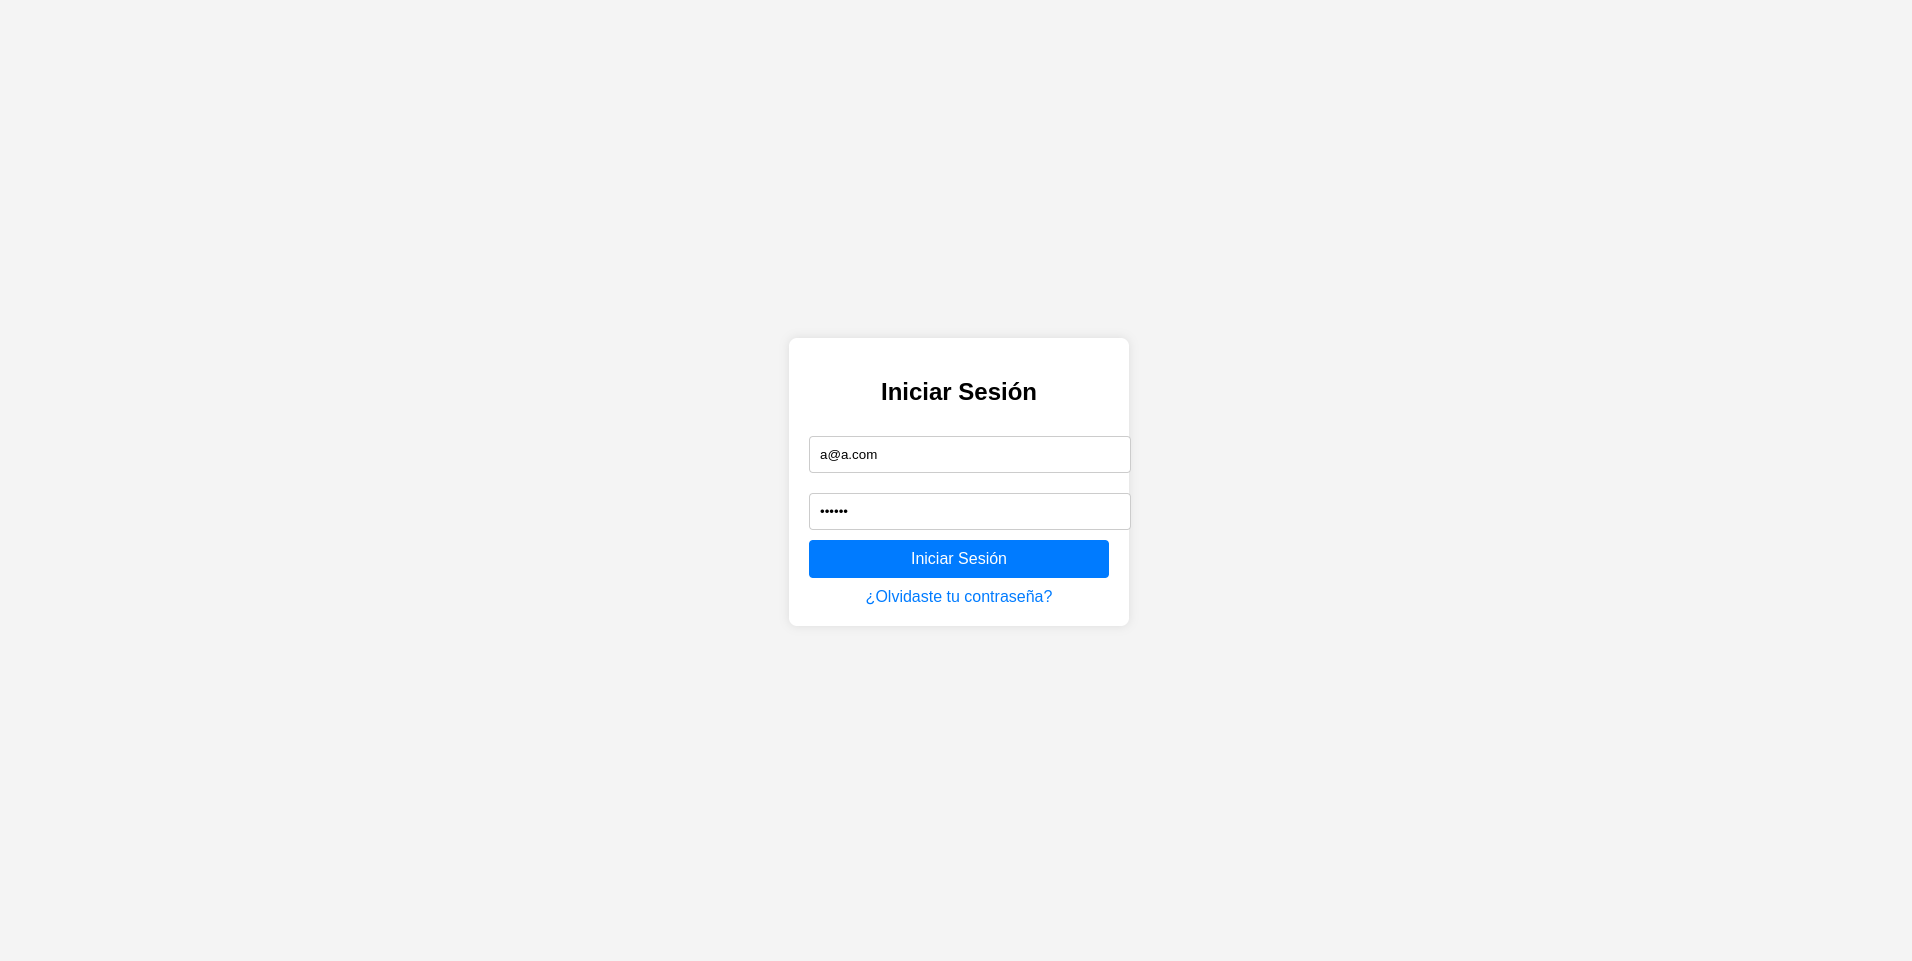
\includegraphics[width=\textwidth]{img/image1.png}
    \caption{Pantalla de Inicio de Sesión: Permite a los usuarios autenticarse ingresando su correo electrónico y contraseña.}
\end{figure}

\begin{figure}[H]
    \centering
    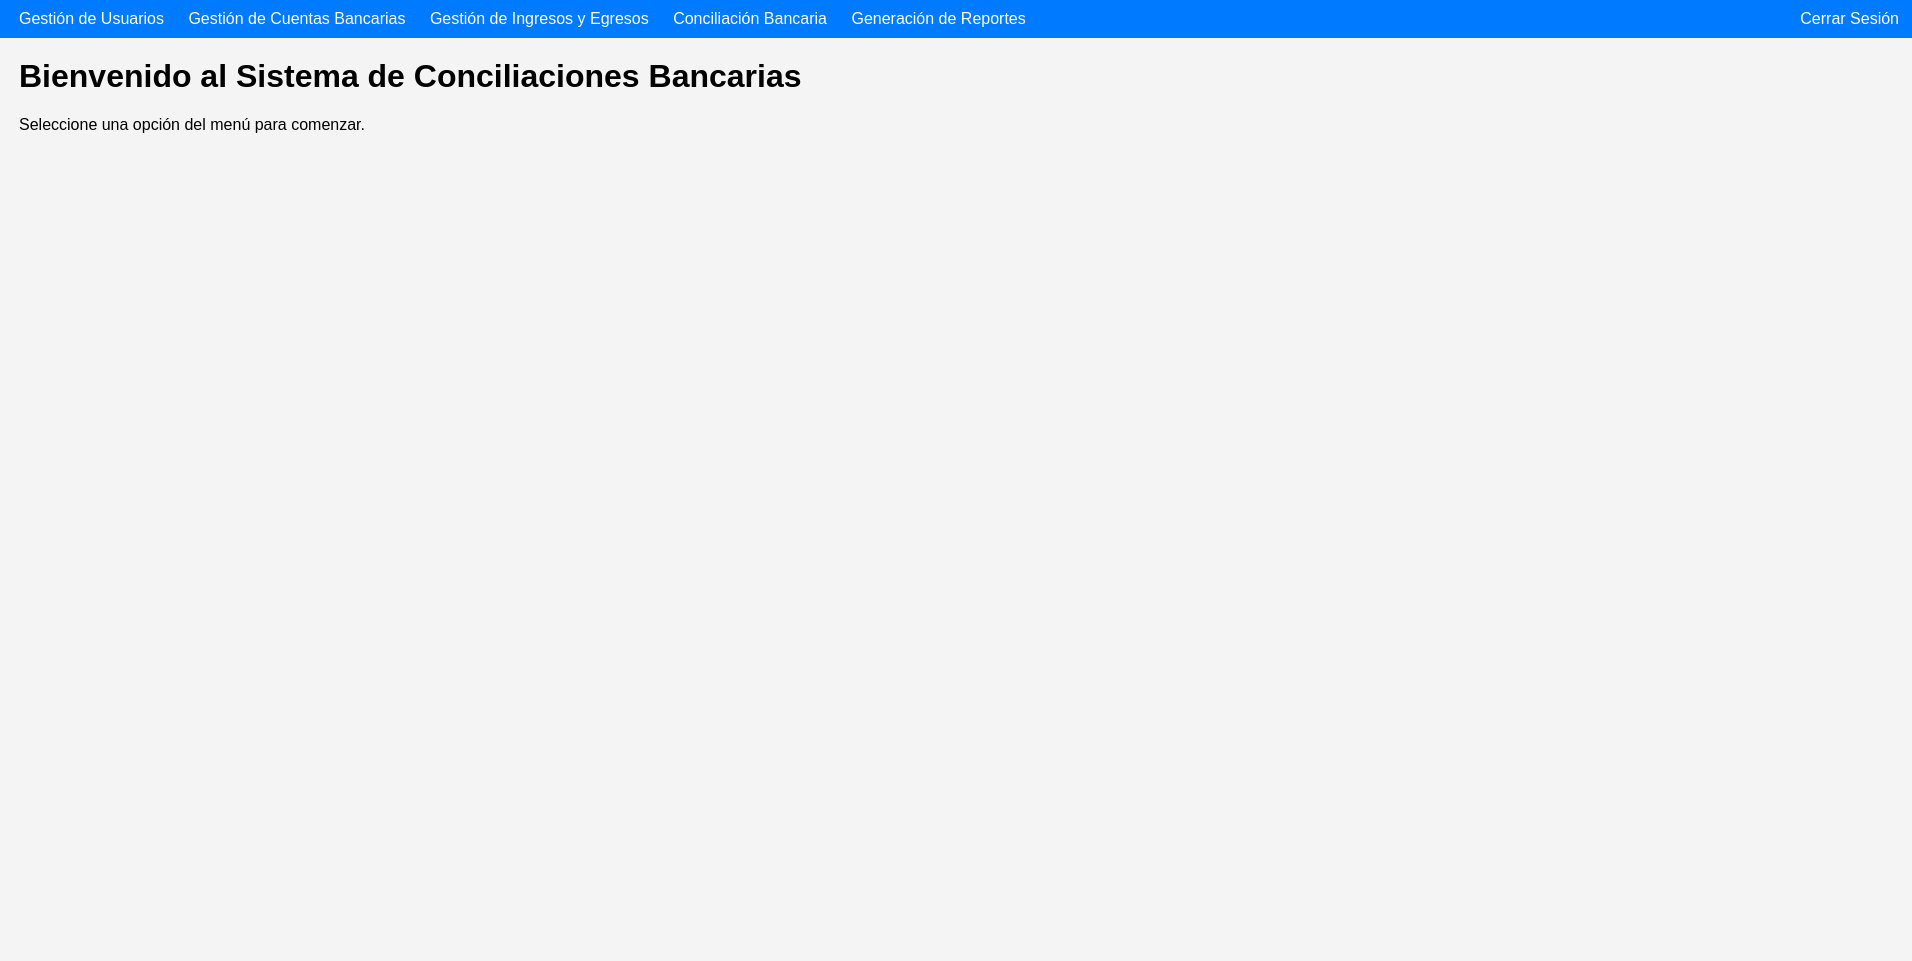
\includegraphics[width=\textwidth]{img/image2.png}
    \caption{Menú Principal: Proporciona acceso a las diferentes funcionalidades del sistema según el rol del usuario.}
\end{figure}

\begin{figure}[H]
    \centering
    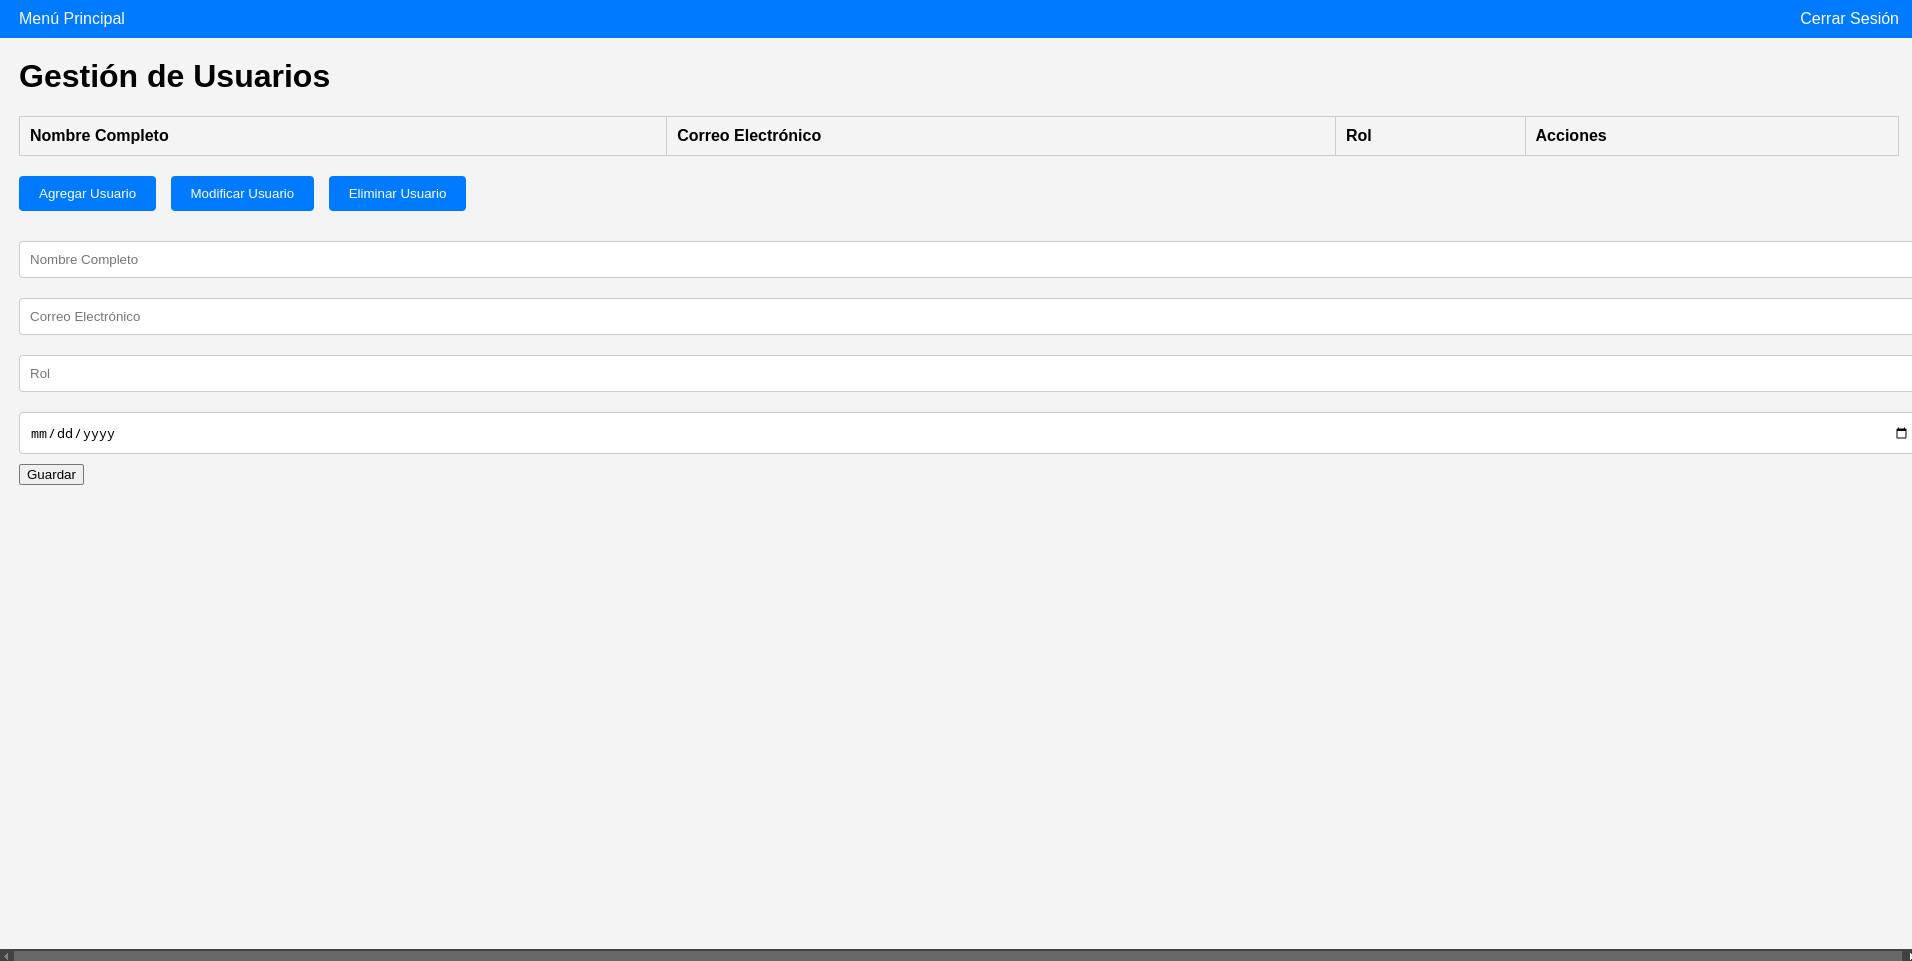
\includegraphics[width=\textwidth]{img/image3.png}
    \caption{Gestión de Usuarios: Permite a los administradores agregar, modificar y eliminar usuarios.}
\end{figure}

\begin{figure}[H]
    \centering
    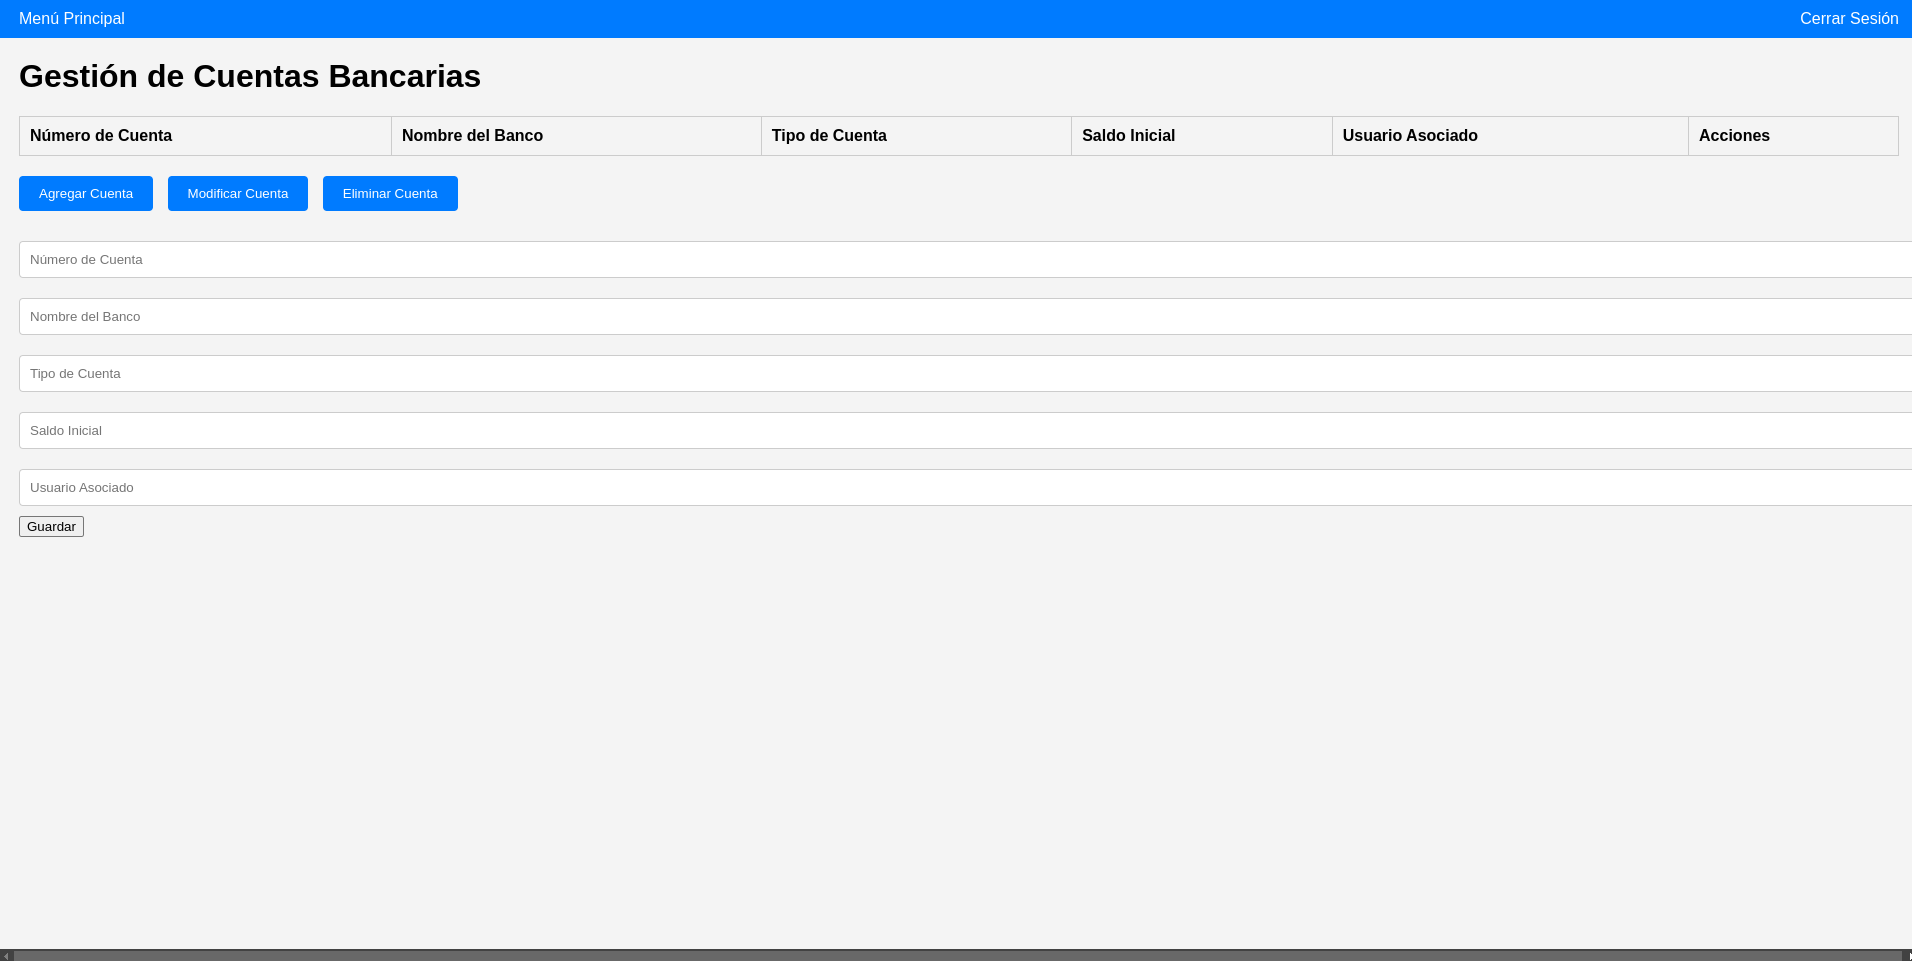
\includegraphics[width=\textwidth]{img/image4.png}
    \caption{Gestión de Cuentas Bancarias: Permite a los administradores agregar, modificar y eliminar cuentas bancarias.}
\end{figure}

\begin{figure}[H]
    \centering
    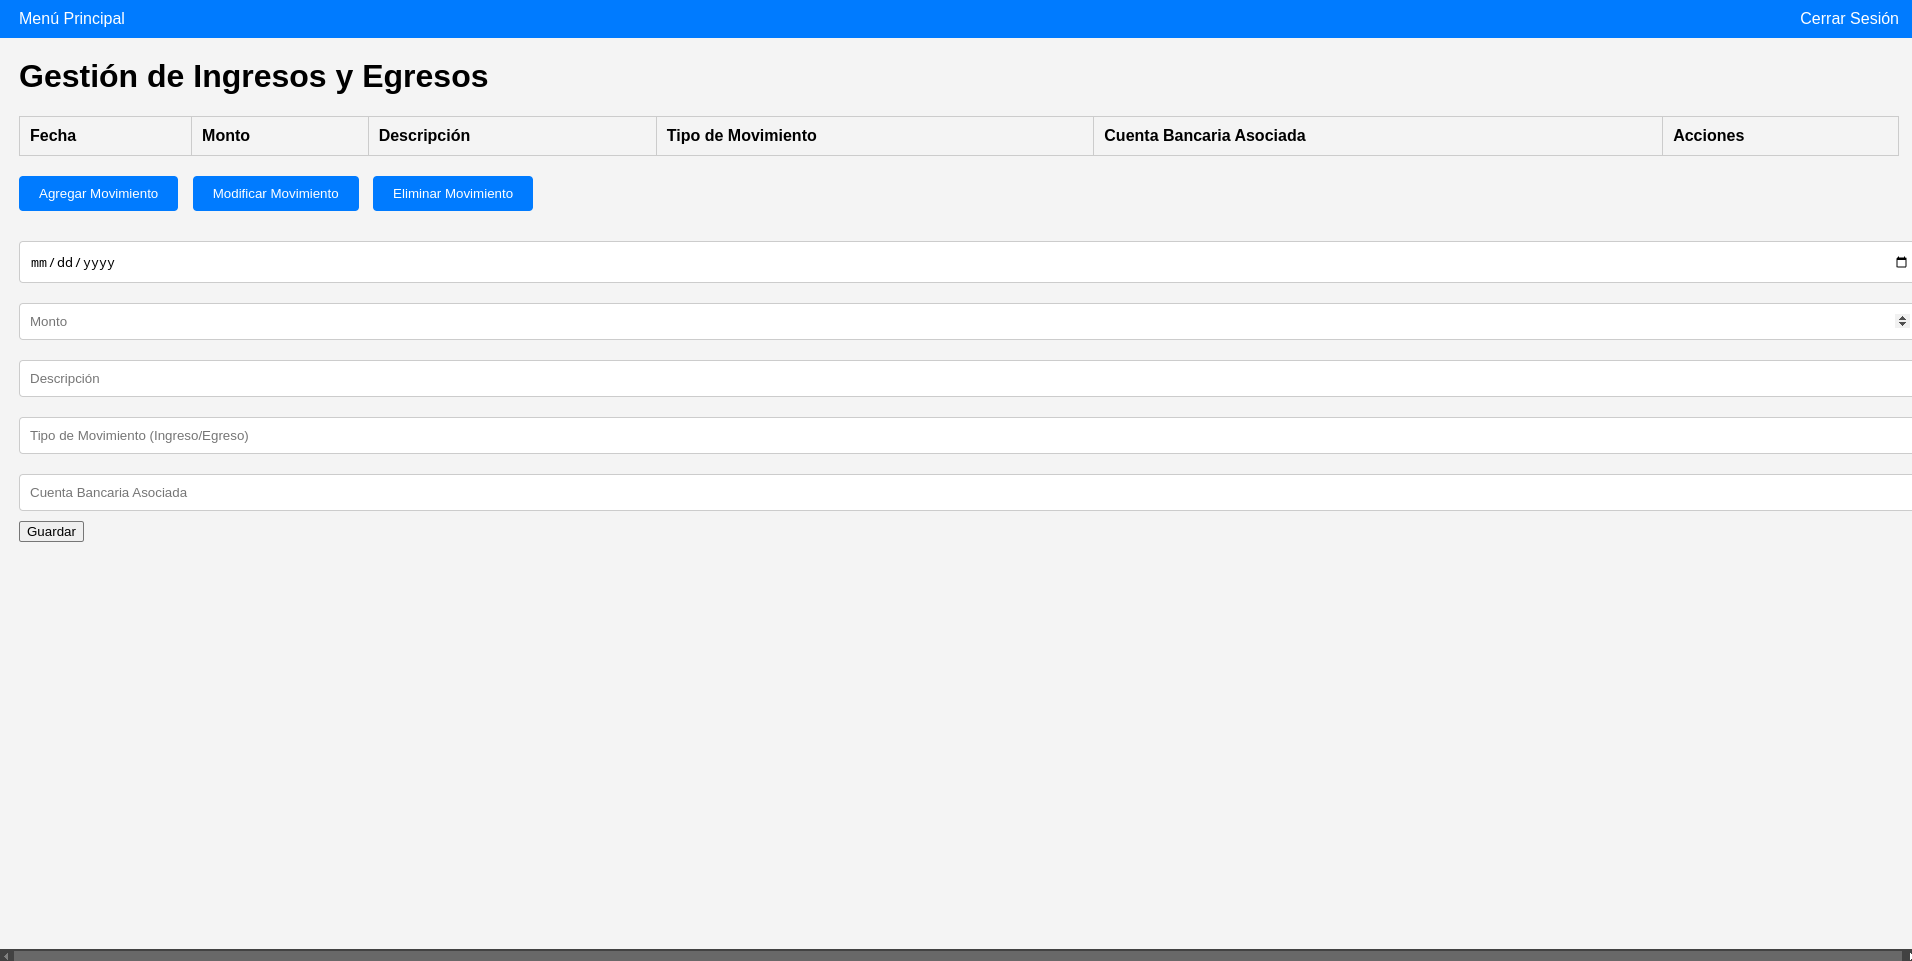
\includegraphics[width=\textwidth]{img/image5.png}
    \caption{Gestión de Ingresos y Egresos: Permite a los administradores y auditores registrar, modificar y eliminar ingresos y egresos.}
\end{figure}

\begin{figure}[H]
    \centering
    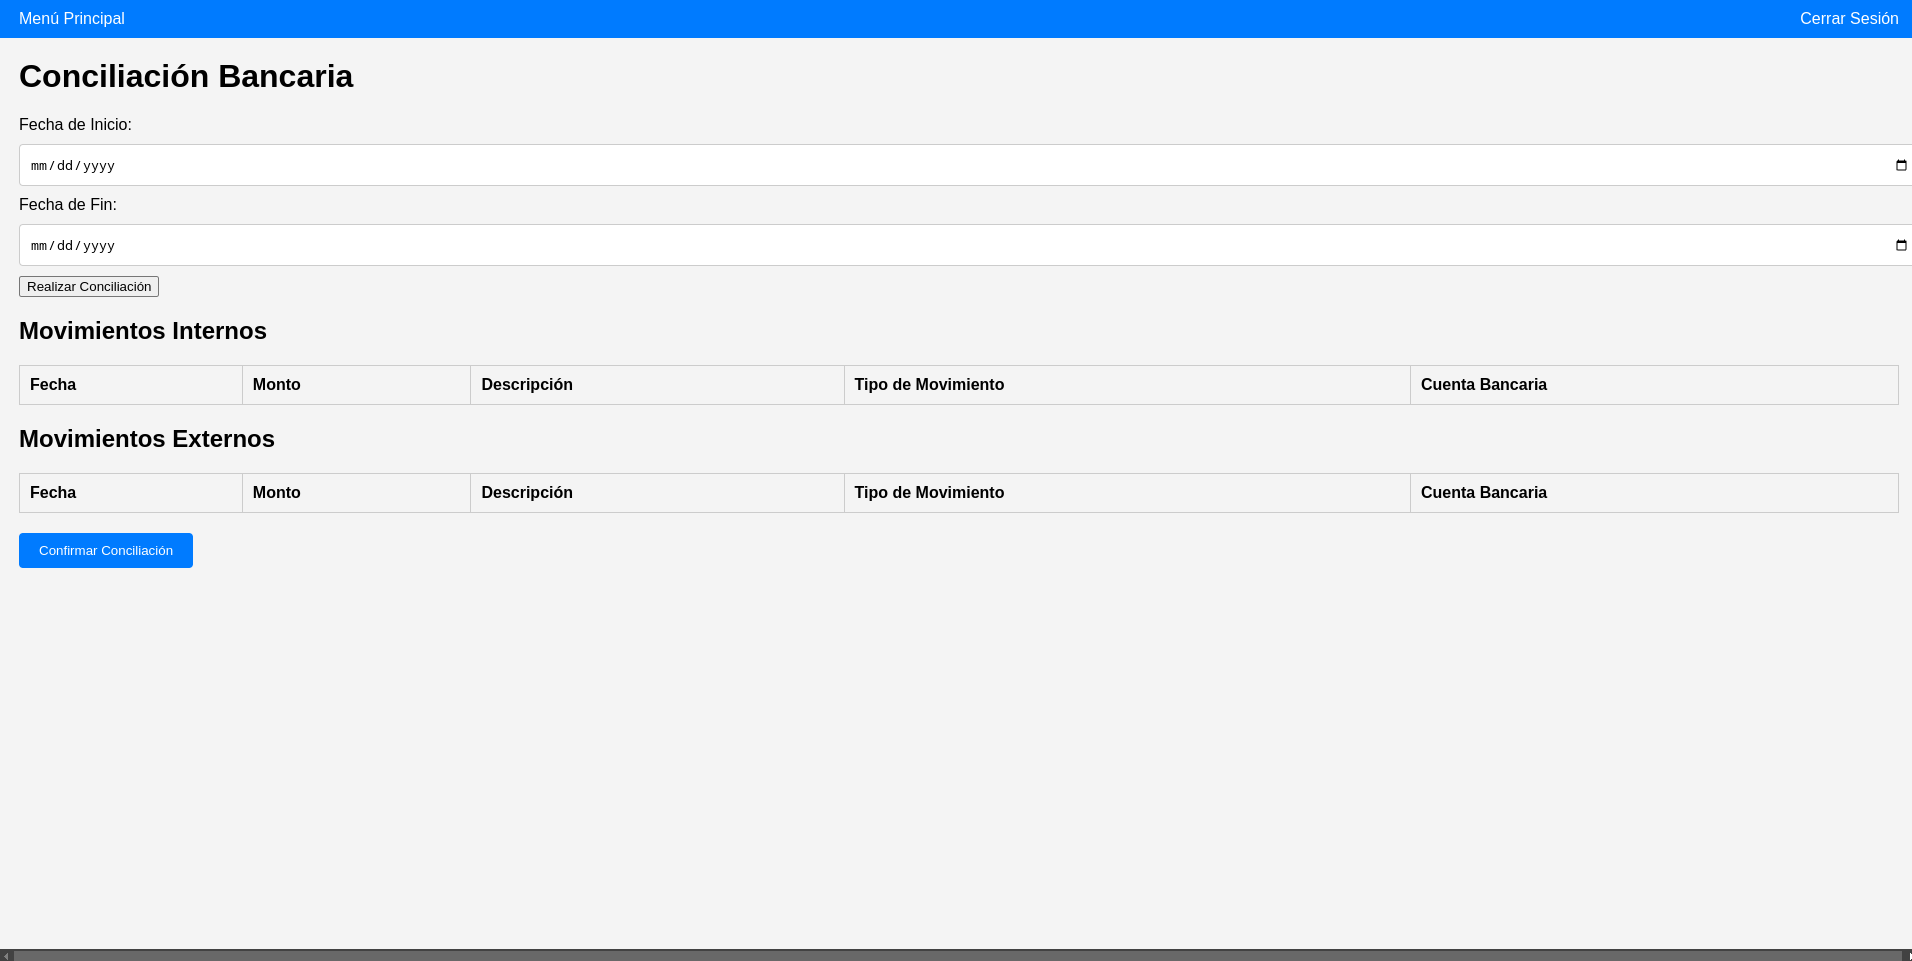
\includegraphics[width=\textwidth]{img/image6.png}
    \caption{Conciliación Bancaria: Permite realizar la conciliación bancaria comparando ingresos y egresos internos con el estado de cuenta bancario.}
\end{figure}

\begin{figure}[H]
    \centering
    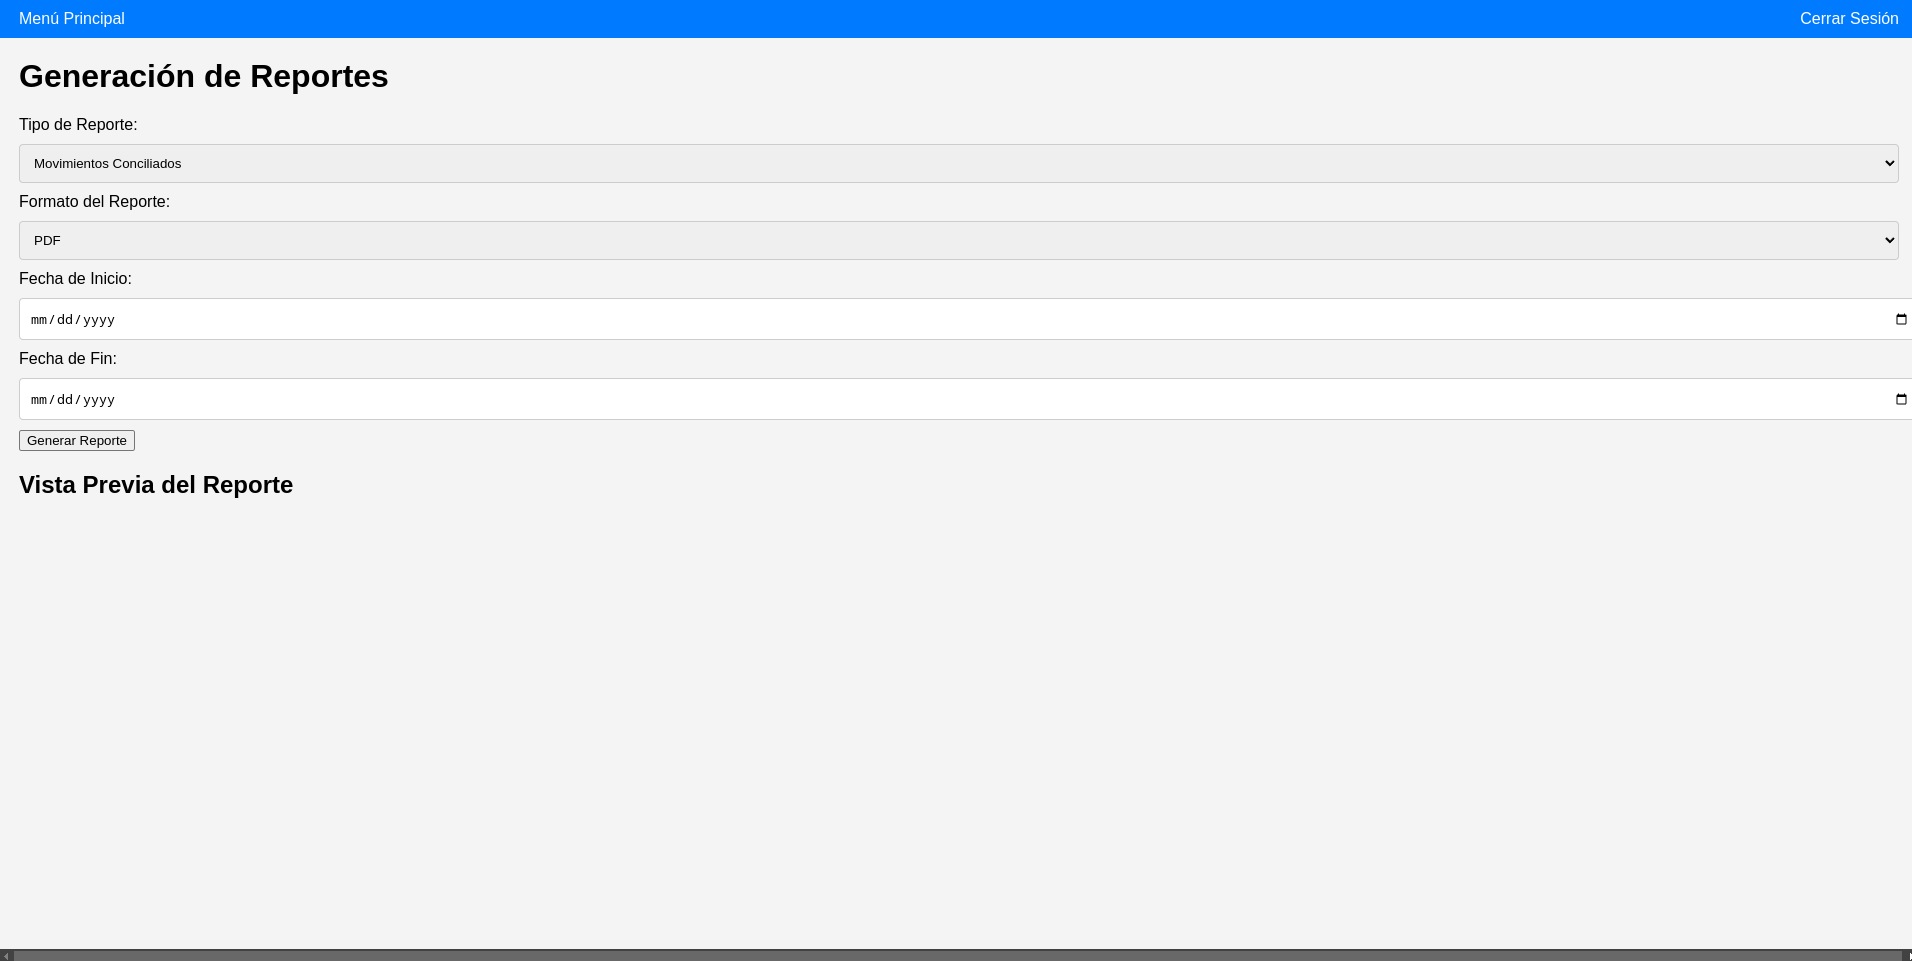
\includegraphics[width=\textwidth]{img/image7.png}
    \caption{Generación de Reportes: Permite a los auditores generar reportes detallados de movimientos conciliados y pendientes.}
\end{figure}

\begin{figure}[H]
    \centering
    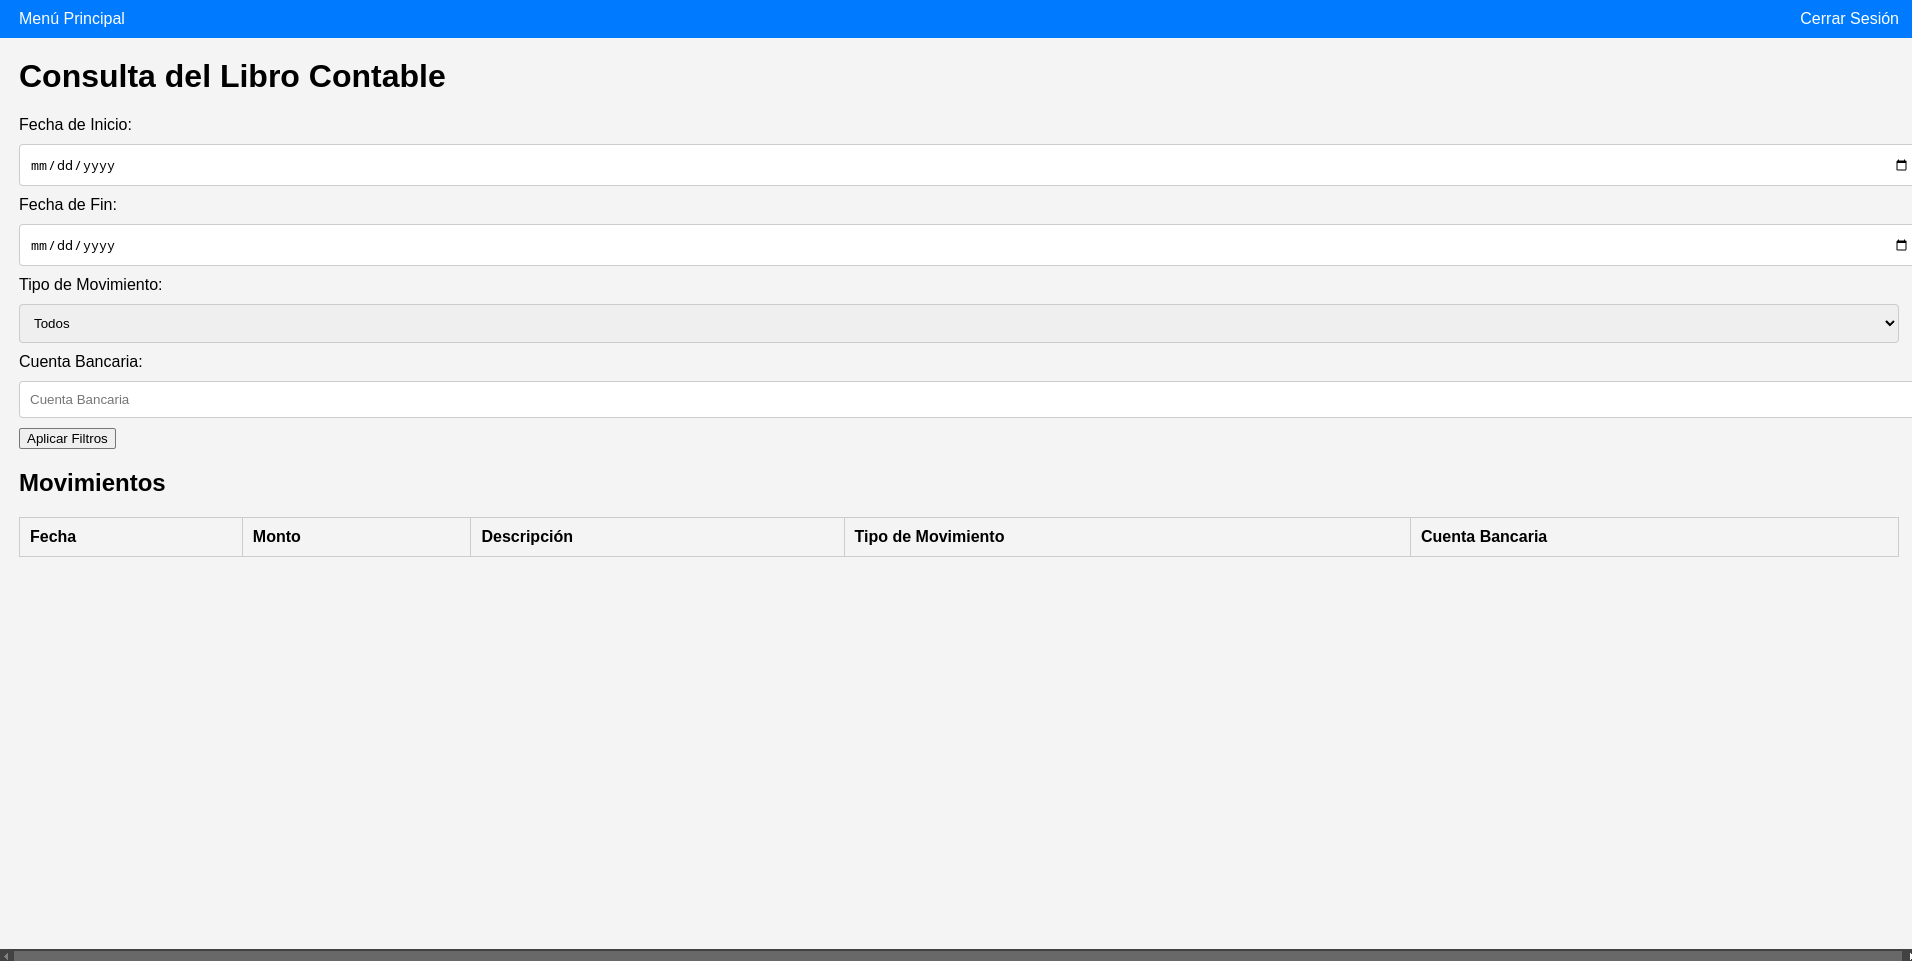
\includegraphics[width=\textwidth]{img/image8.png}
    \caption{Consulta del Libro Contable: Permite a los administradores y auditores consultar el libro contable aplicando filtros.}
\end{figure}

\begin{figure}[H]
    \centering
    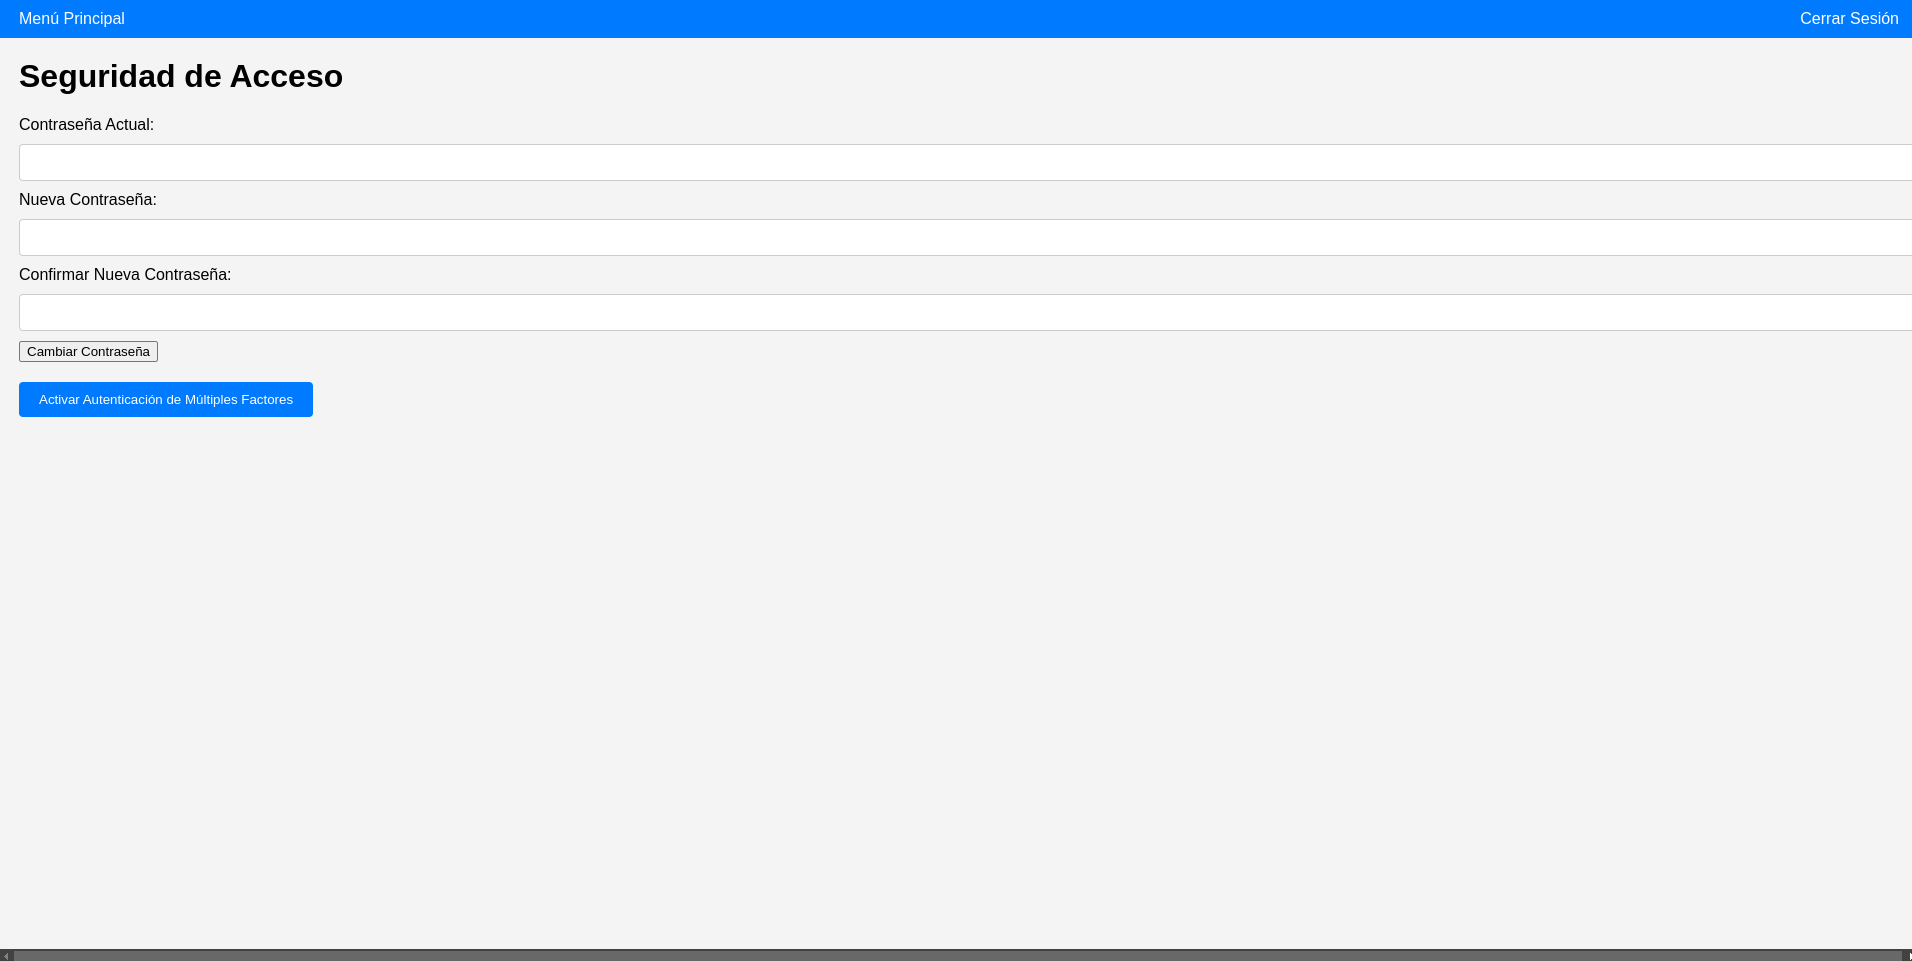
\includegraphics[width=\textwidth]{img/image9.png}
    \caption{Seguridad de Acceso: Permite a los usuarios cambiar su contraseña y activar la autenticación de múltiples factores.}
\end{figure}

\subsection{Diagrama de Casos de Uso}

\begin{figure}[H]
    \centering
    % 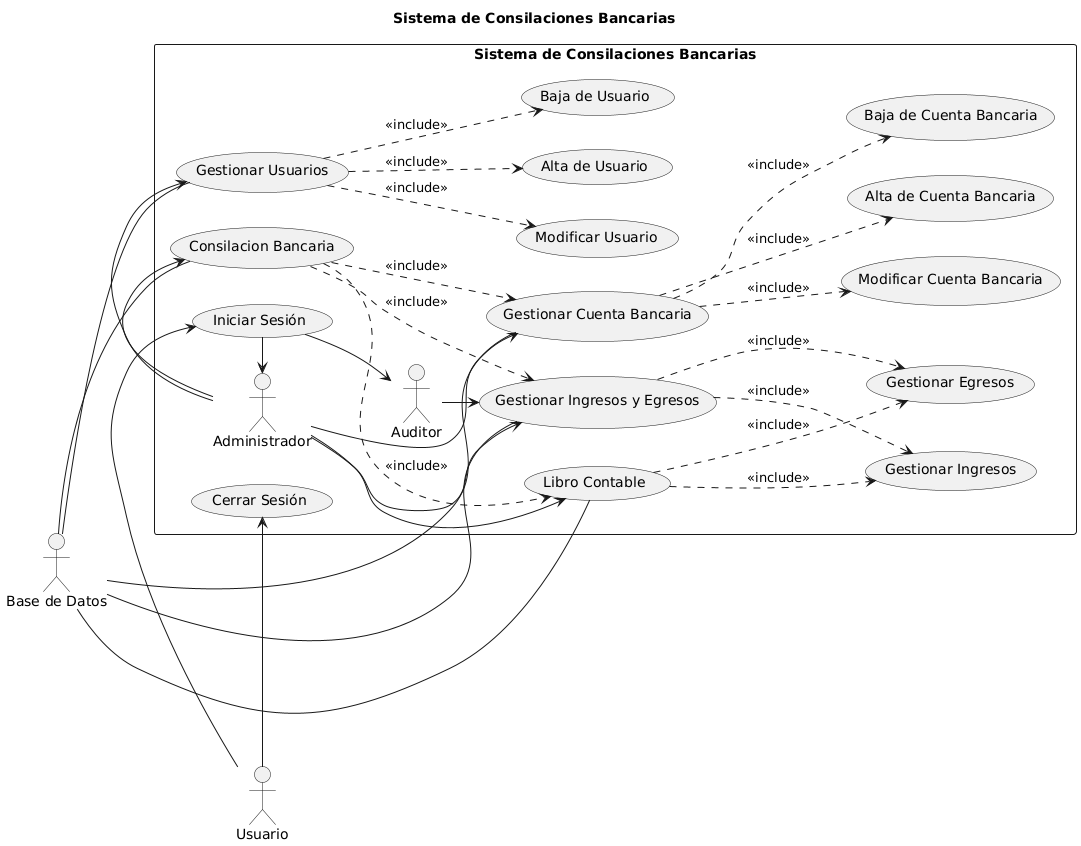
\includegraphics[width=\textwidth]{casos/UML-General.png}
    \caption{Diagrama General de Casos de Uso del Proyecto: Muestra las interacciones entre los actores y los casos de uso del sistema.}
\end{figure}

\begin{figure}[H]
    \centering
    % 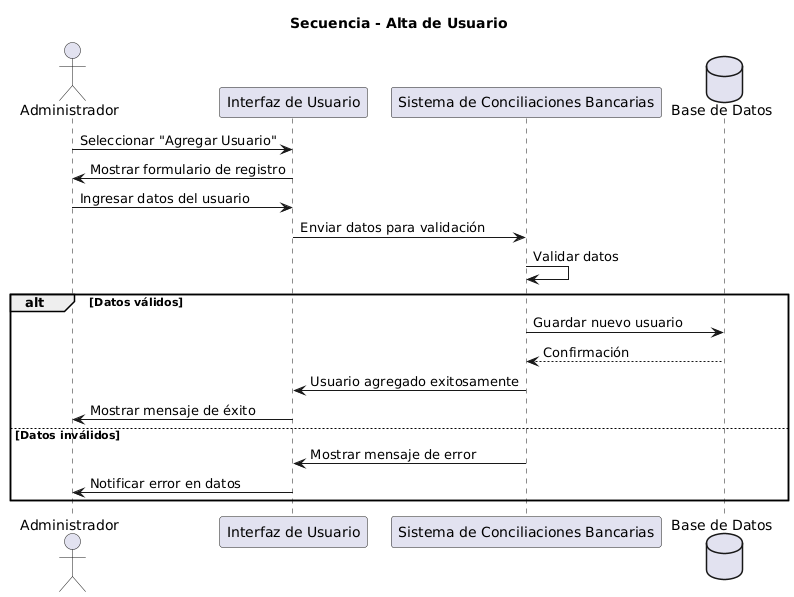
\includegraphics[width=\textwidth]{casos/AltaDeUsuario.png}
    \caption{Diagrama de Secuencia: Alta de Usuario}
\end{figure}

\begin{figure}[H]
    \centering
    % 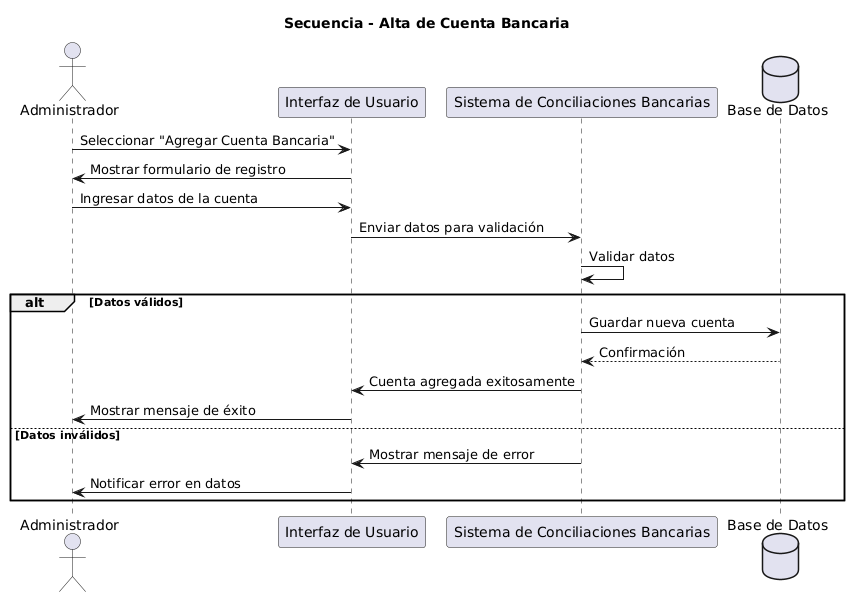
\includegraphics[width=\textwidth]{casos/AltaDeCuentaBancaria.png}
    \caption{Diagrama de Secuencia: Alta de Cuenta Bancaria}
\end{figure}

\begin{figure}[H]
    \centering
    % 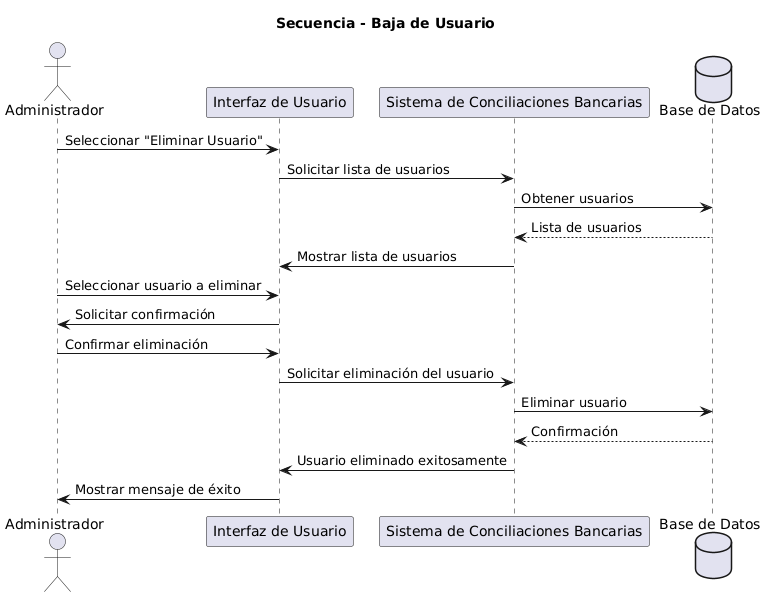
\includegraphics[width=\textwidth]{casos/BajaDeUsuario.png}
    \caption{Diagrama de Secuencia: Baja de Usuario}
\end{figure}

\begin{figure}[H]
    \centering
    % 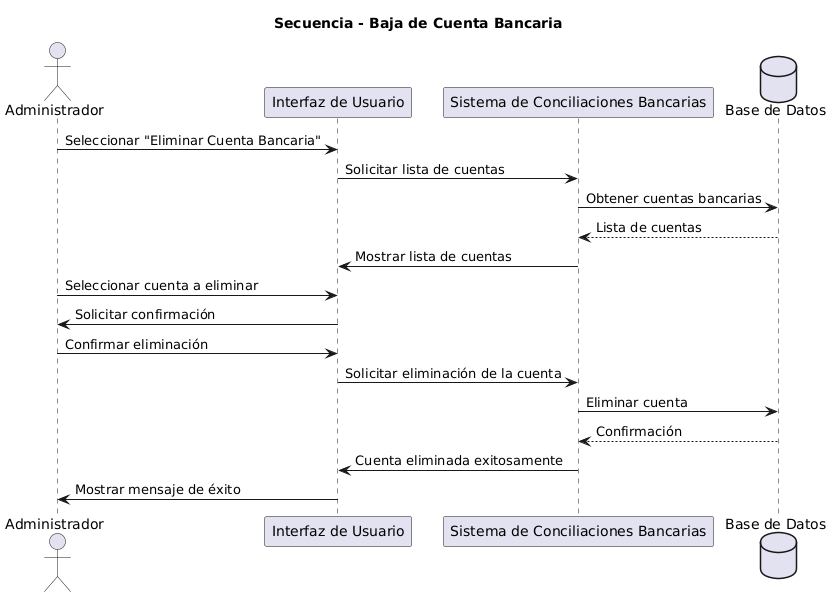
\includegraphics[width=\textwidth]{casos/BajaDeCuentaBancaria.png}
    \caption{Diagrama de Secuencia: Baja de Cuenta Bancaria}
\end{figure}

\begin{figure}[H]
    \centering
    % 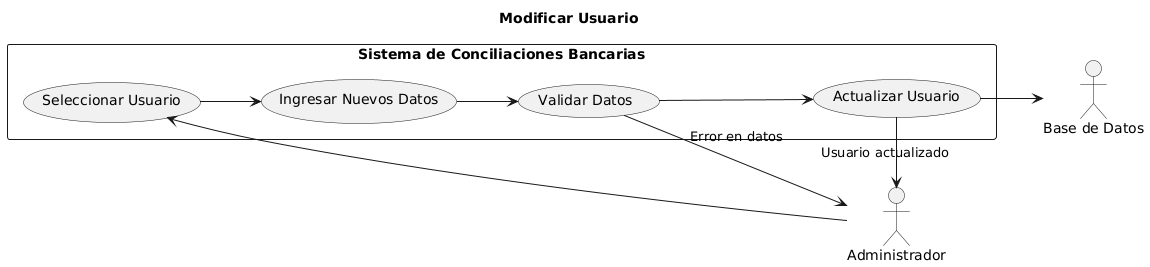
\includegraphics[width=\textwidth]{casos/ModificarUsuario.png}
    \caption{Diagrama de Secuencia: Modificar Usuario}
\end{figure}

\begin{figure}[H]
    \centering
    % 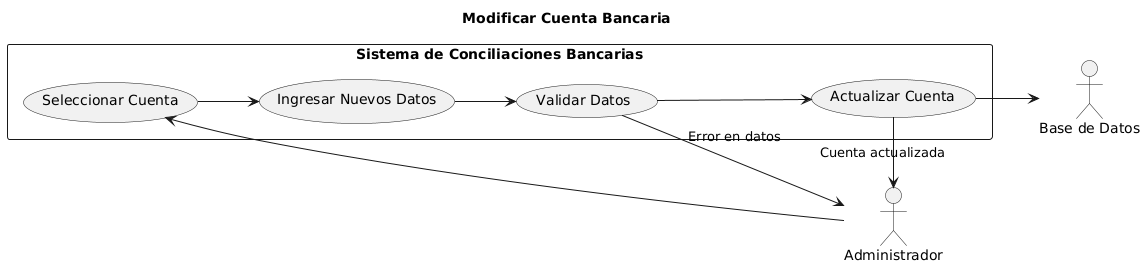
\includegraphics[width=\textwidth]{casos/ModificarCuentaBancaria.png}
    \caption{Diagrama de Secuencia: Modificar Cuenta Bancaria}
\end{figure}

\begin{figure}[H]
    \centering
    % 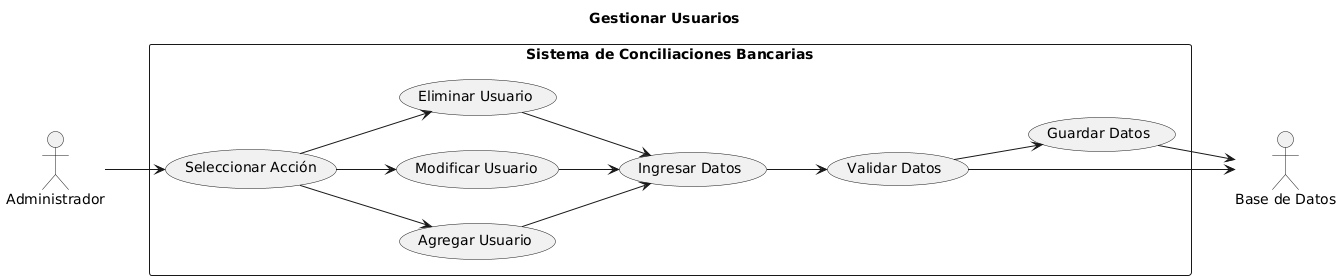
\includegraphics[width=\textwidth]{casos/GestionarUsuarios.png}
    \caption{Diagrama de Secuencia: Gestionar Usuarios}
\end{figure}

\begin{figure}[H]
    \centering
    % 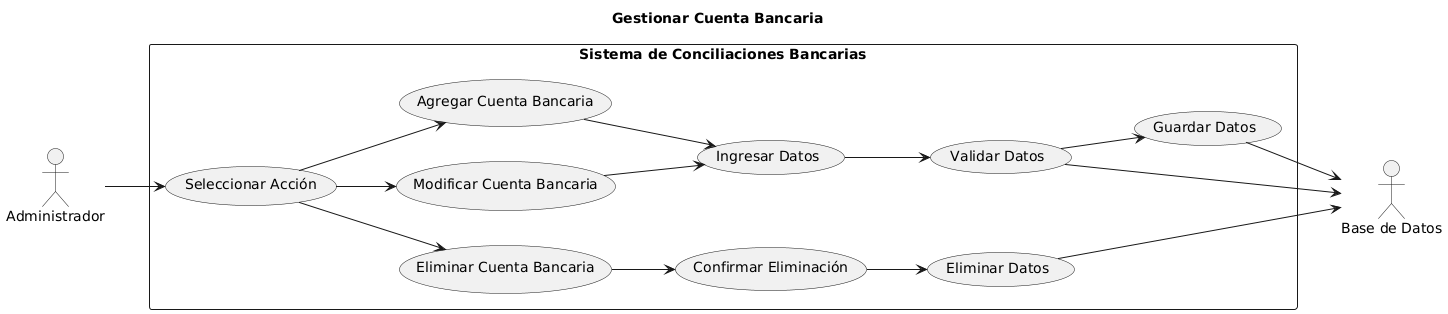
\includegraphics[width=\textwidth]{casos/GestionarCuentaBancaria.png}
    \caption{Diagrama de Secuencia: Gestionar Cuenta Bancaria}
\end{figure}

\begin{figure}[H]
    \centering
    % 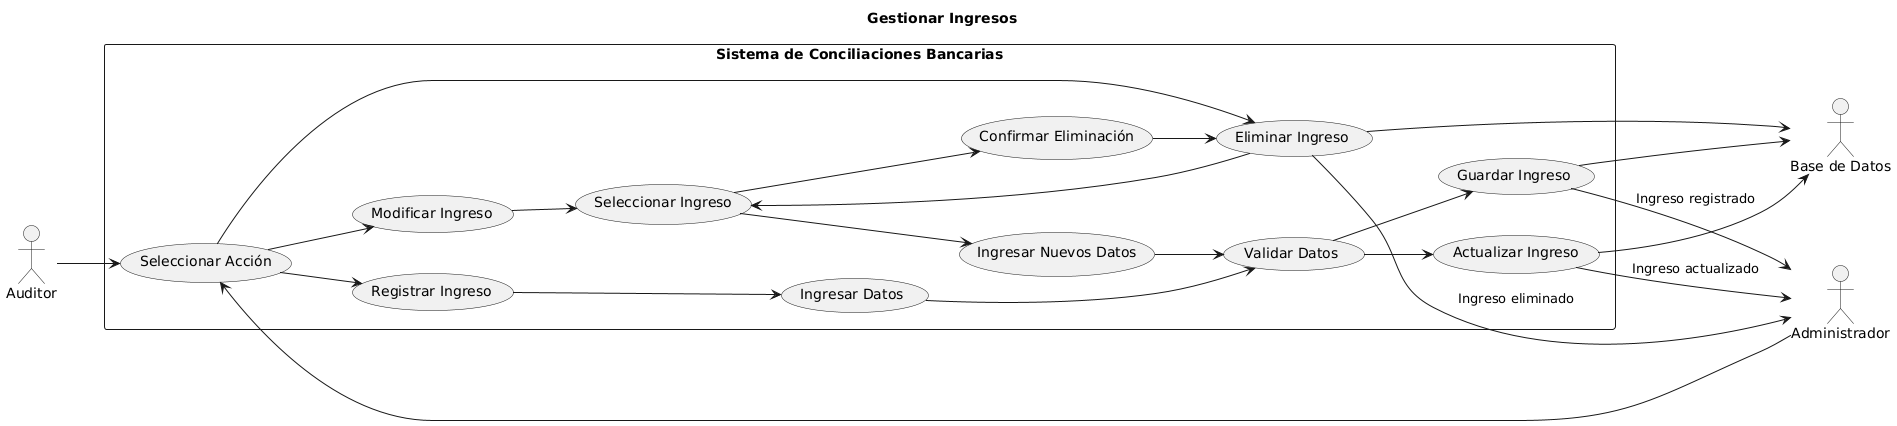
\includegraphics[width=\textwidth]{casos/GestionarIngresos.png}
    \caption{Diagrama de Secuencia: Gestionar Ingresos}
\end{figure}

\begin{figure}[H]
    \centering
    % 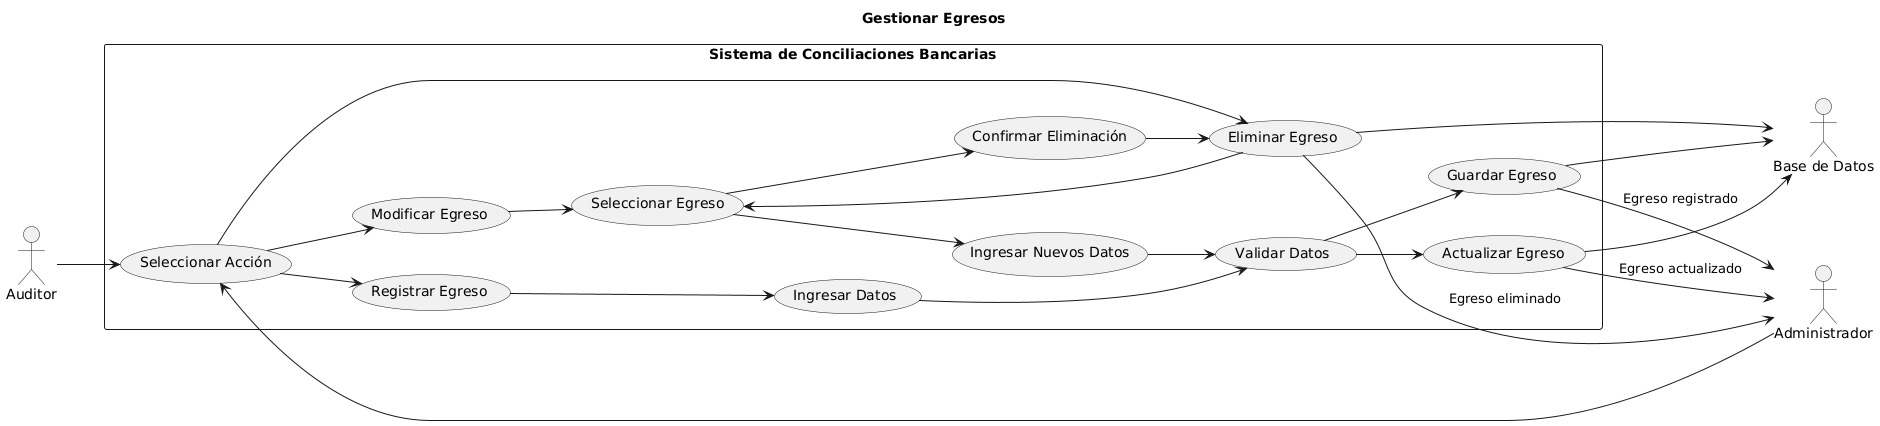
\includegraphics[width=\textwidth]{casos/GestionarEgresos.png}
    \caption{Diagrama de Secuencia: Gestionar Egresos}
\end{figure}

\begin{figure}[H]
    \centering
    % 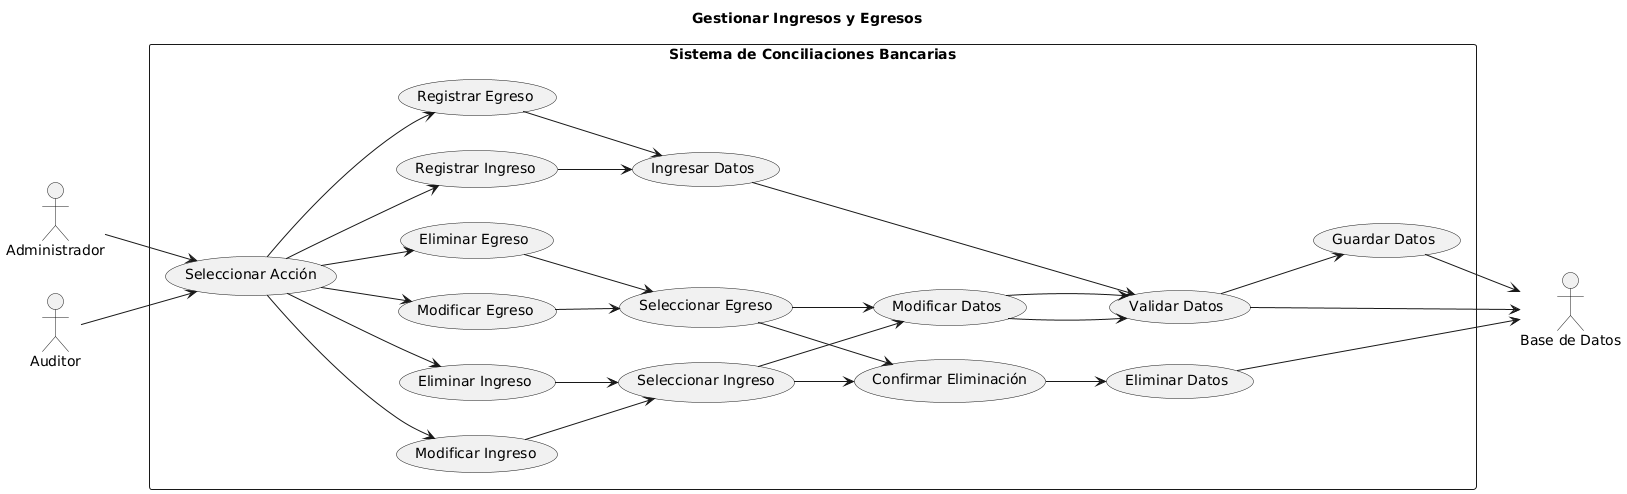
\includegraphics[width=\textwidth]{casos/GestionarIngresosEgresos.png}
    \caption{Diagrama de Secuencia: Gestionar Ingresos y Egresos}
\end{figure}

\begin{figure}[H]
    \centering
    % 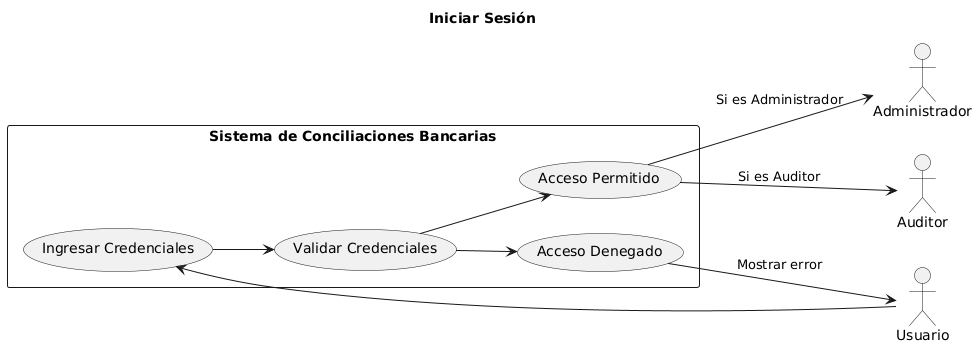
\includegraphics[width=\textwidth]{casos/IniciarSesion.png}
    \caption{Diagrama de Secuencia: Iniciar Sesión}
\end{figure}

\begin{figure}[H]
    \centering
    % 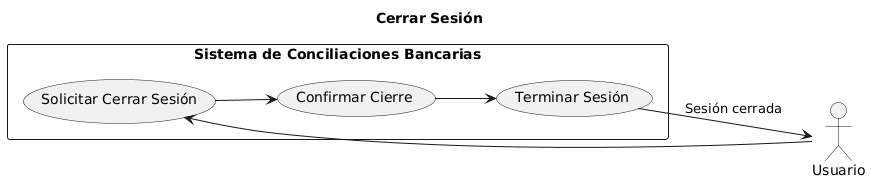
\includegraphics[width=\textwidth]{casos/CerrarSesion.png}
    \caption{Diagrama de Secuencia: Cerrar Sesión}
\end{figure}

\begin{figure}[H]
    \centering
    % 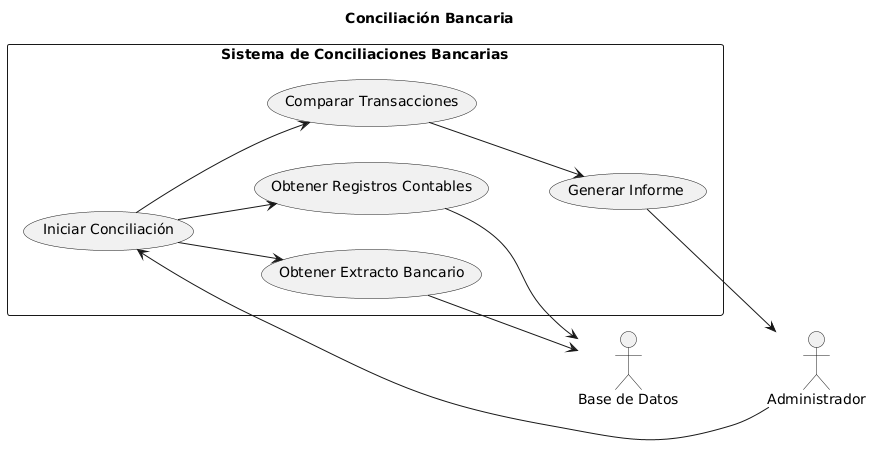
\includegraphics[width=\textwidth]{casos/ConciliacionBancaria.png}
    \caption{Diagrama de Secuencia: Conciliación Bancaria}
\end{figure}

\begin{figure}[H]
    \centering
    % 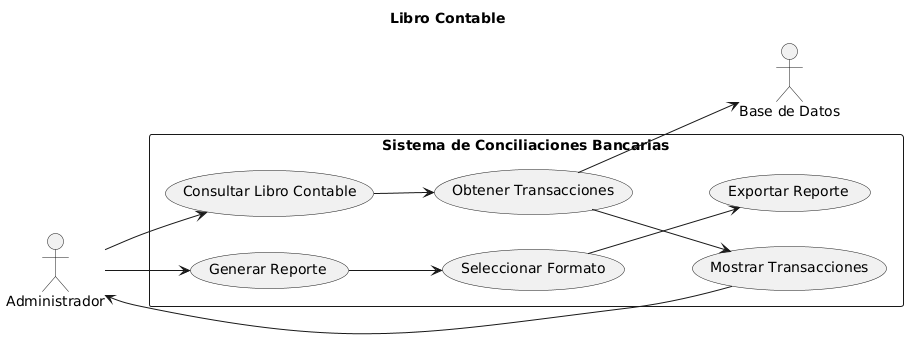
\includegraphics[width=\textwidth]{casos/LibroContable.png}
    \caption{Diagrama de Secuencia: Libro Contable}
\end{figure}

\subsection{Diagrama Entidad-Relación}
\begin{figure}[H]
    \centering
    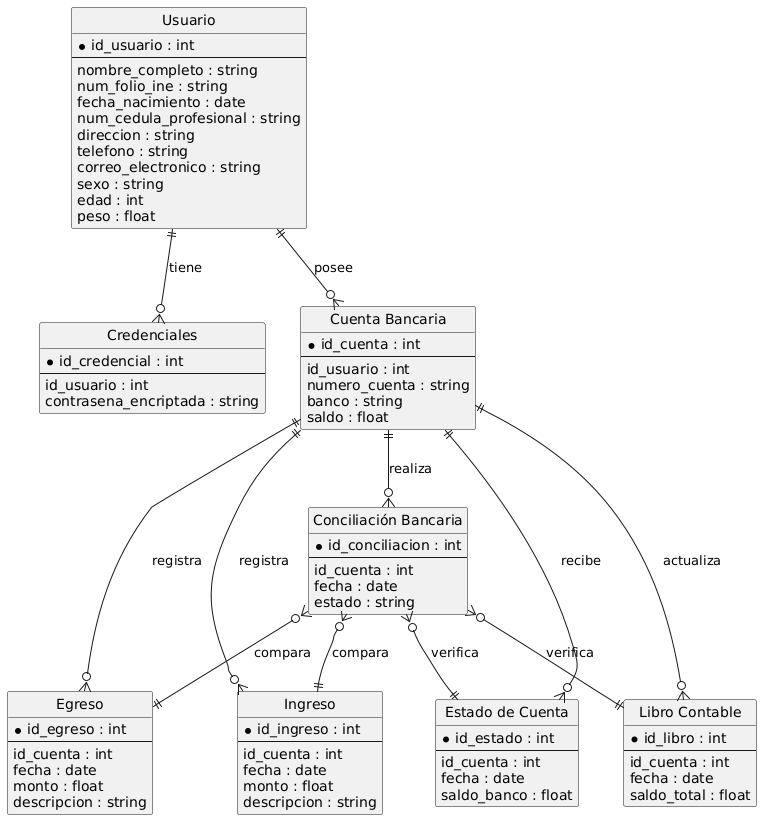
\includegraphics[width=\textwidth]{casos/EntidadRelacion.png}
    \caption{Diagrama Entidad-Relación del Sistema: Muestra las entidades y relaciones principales del sistema.}
\end{figure}

\end{document}